\chapter{Dependencies of $\mathbf{R}_{\text{out/in}}$}
In addition to the results for the low-mass region already shown in Section~\ref{sec:ROutIn}, the dependency of \Routin on \MET and \njets is also studied for the high-mass region. The corresponding results are shown in Figure~\ref{fig:ROutInDependencies2}. As for the low-mass region, no significant dependencies are observed, except in the case of the \MET dependency in the forward region, where a trend to higher values can be seen above $\unit{40}{\giga\electronvolt}$, although with large statistical uncertainties. Also, for the high mass region the flavour-symmetric backgrounds are a significant contribution to the event sample above this value of \MET and therefore the measurement is highly susceptible to the subtraction of this background based on OF events. Similar results are observed for both the low-mass and high-mass region when the event sample is split in to \EE and \MM lepton pairs, as shown in Figures~\ref{fig:ROutInDependencies3}-\ref{fig:ROutInDependencies6}.
\label{app:routin}
\begin{figure}[htbp]
\centering
\begin{minipage}[t]{0.49\textwidth}
  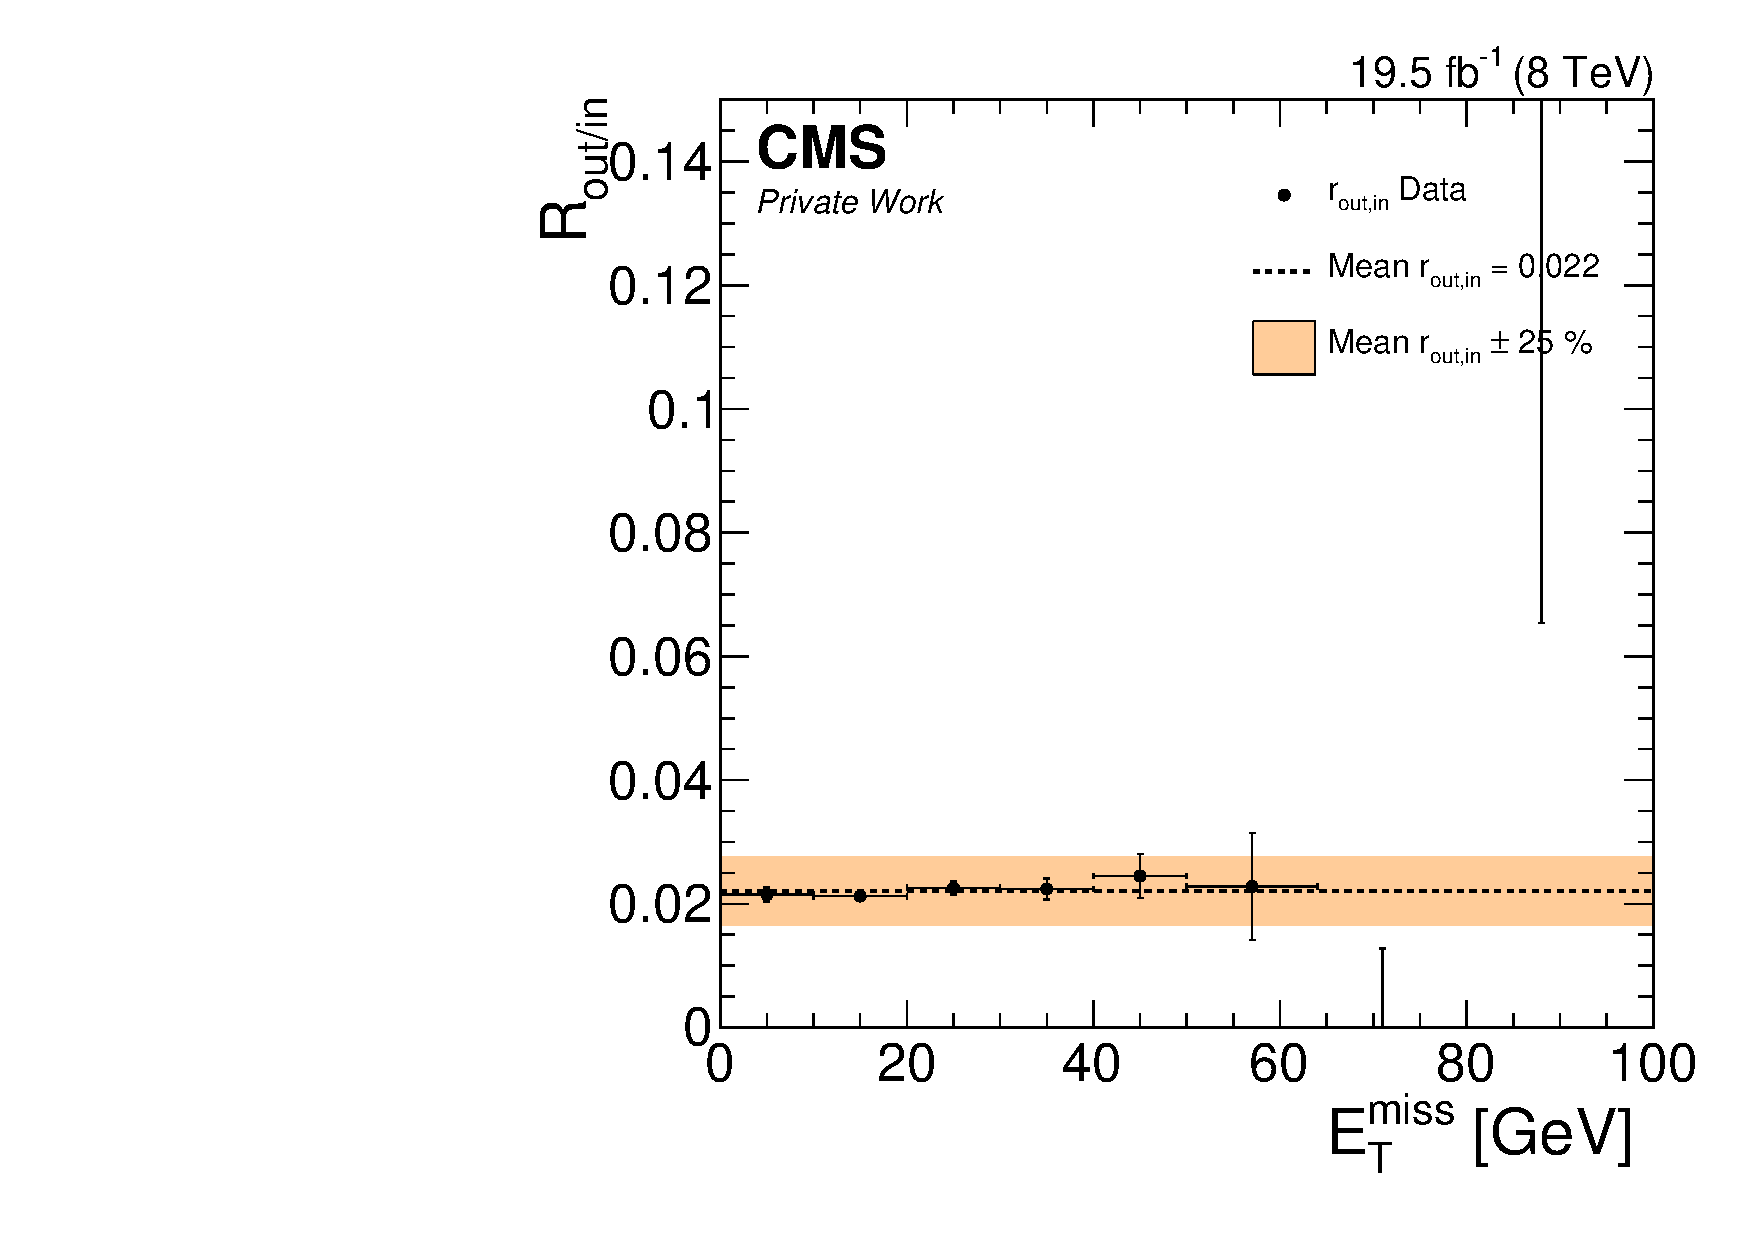
\includegraphics[width=\textwidth]{plots/BG/rOutIn/rOutInSyst_DrellYanControlCentral_Full2012_MET_HighMass_SF_None.pdf}
\end{minipage}
\begin{minipage}[t]{0.49\textwidth}
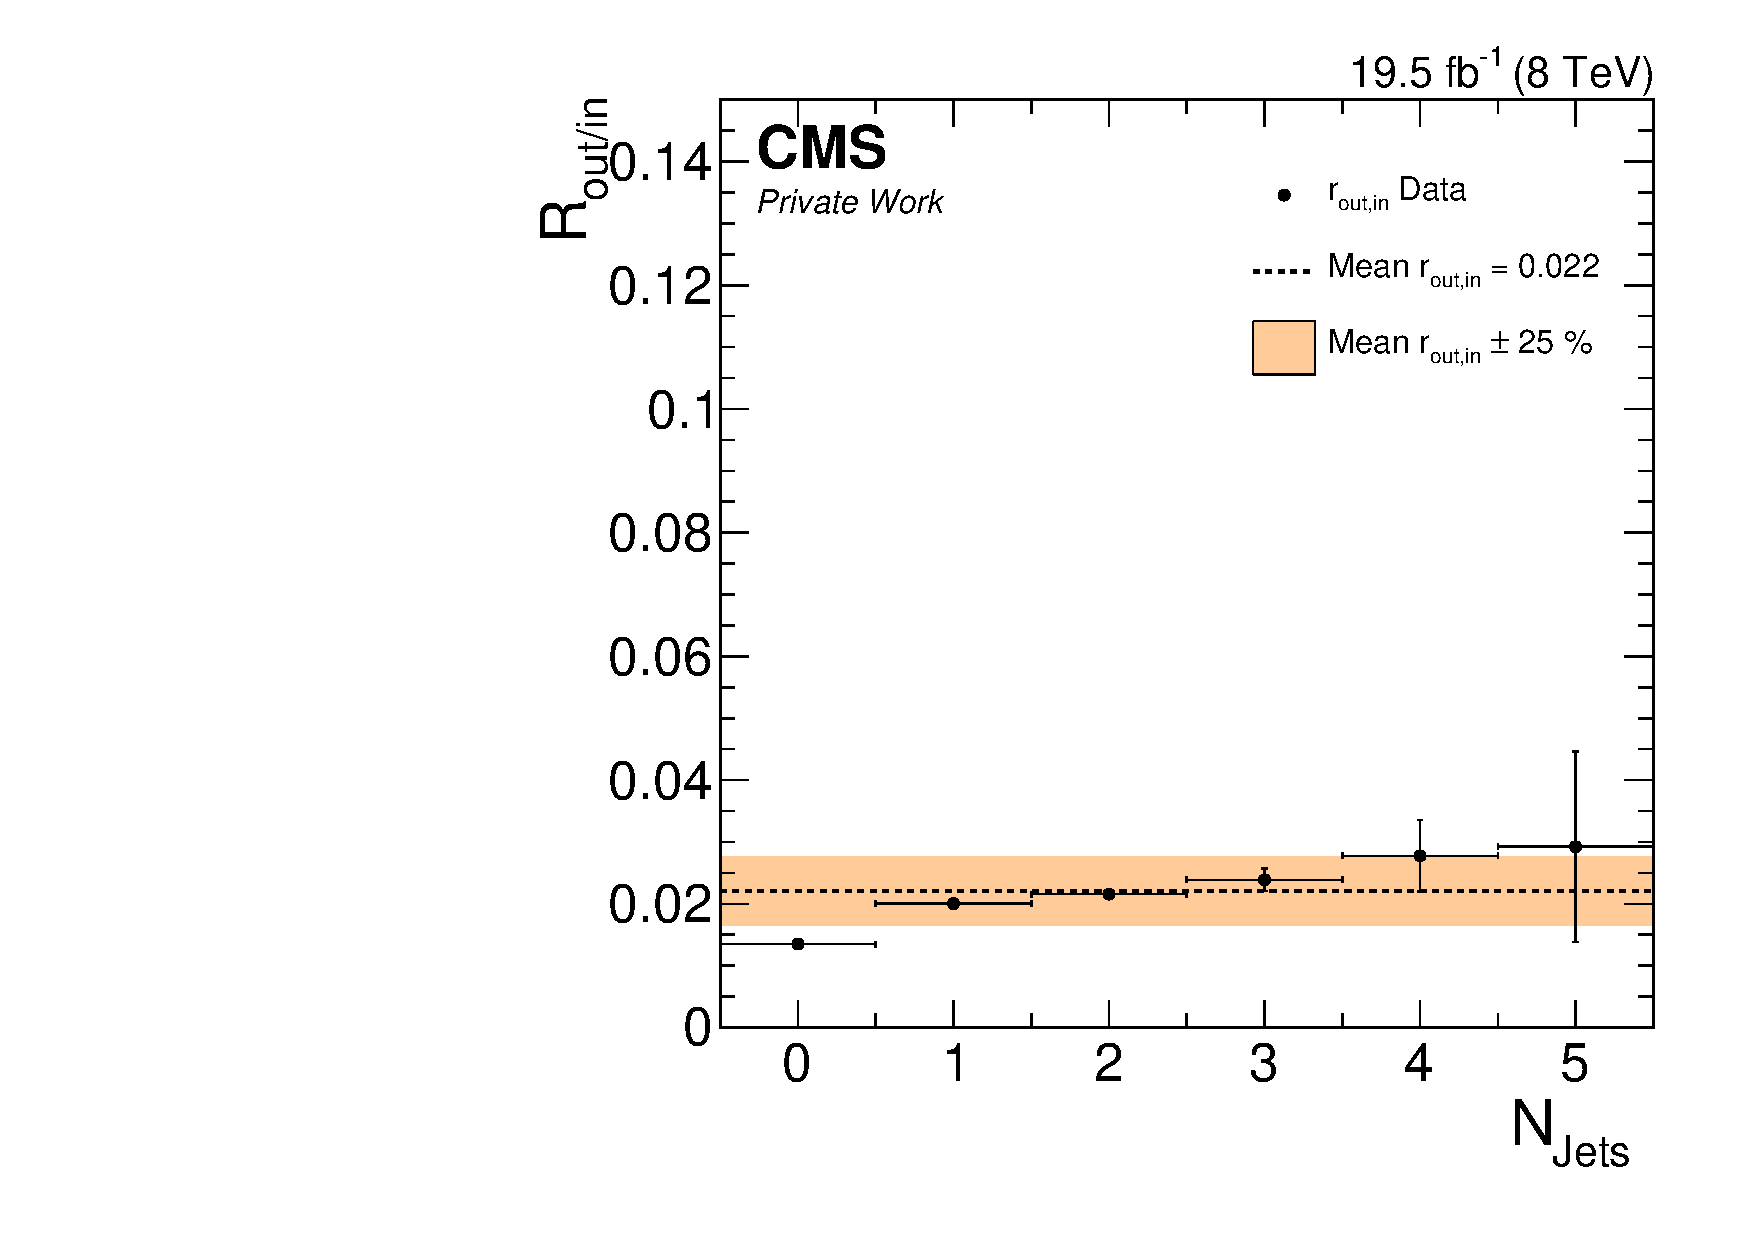
\includegraphics[width=\textwidth]{plots/BG/rOutIn/rOutInSyst_DrellYanControlCentral_Full2012_NJets_HighMass_SF_None.pdf}
\end{minipage}
\begin{minipage}[t]{0.49\textwidth}
  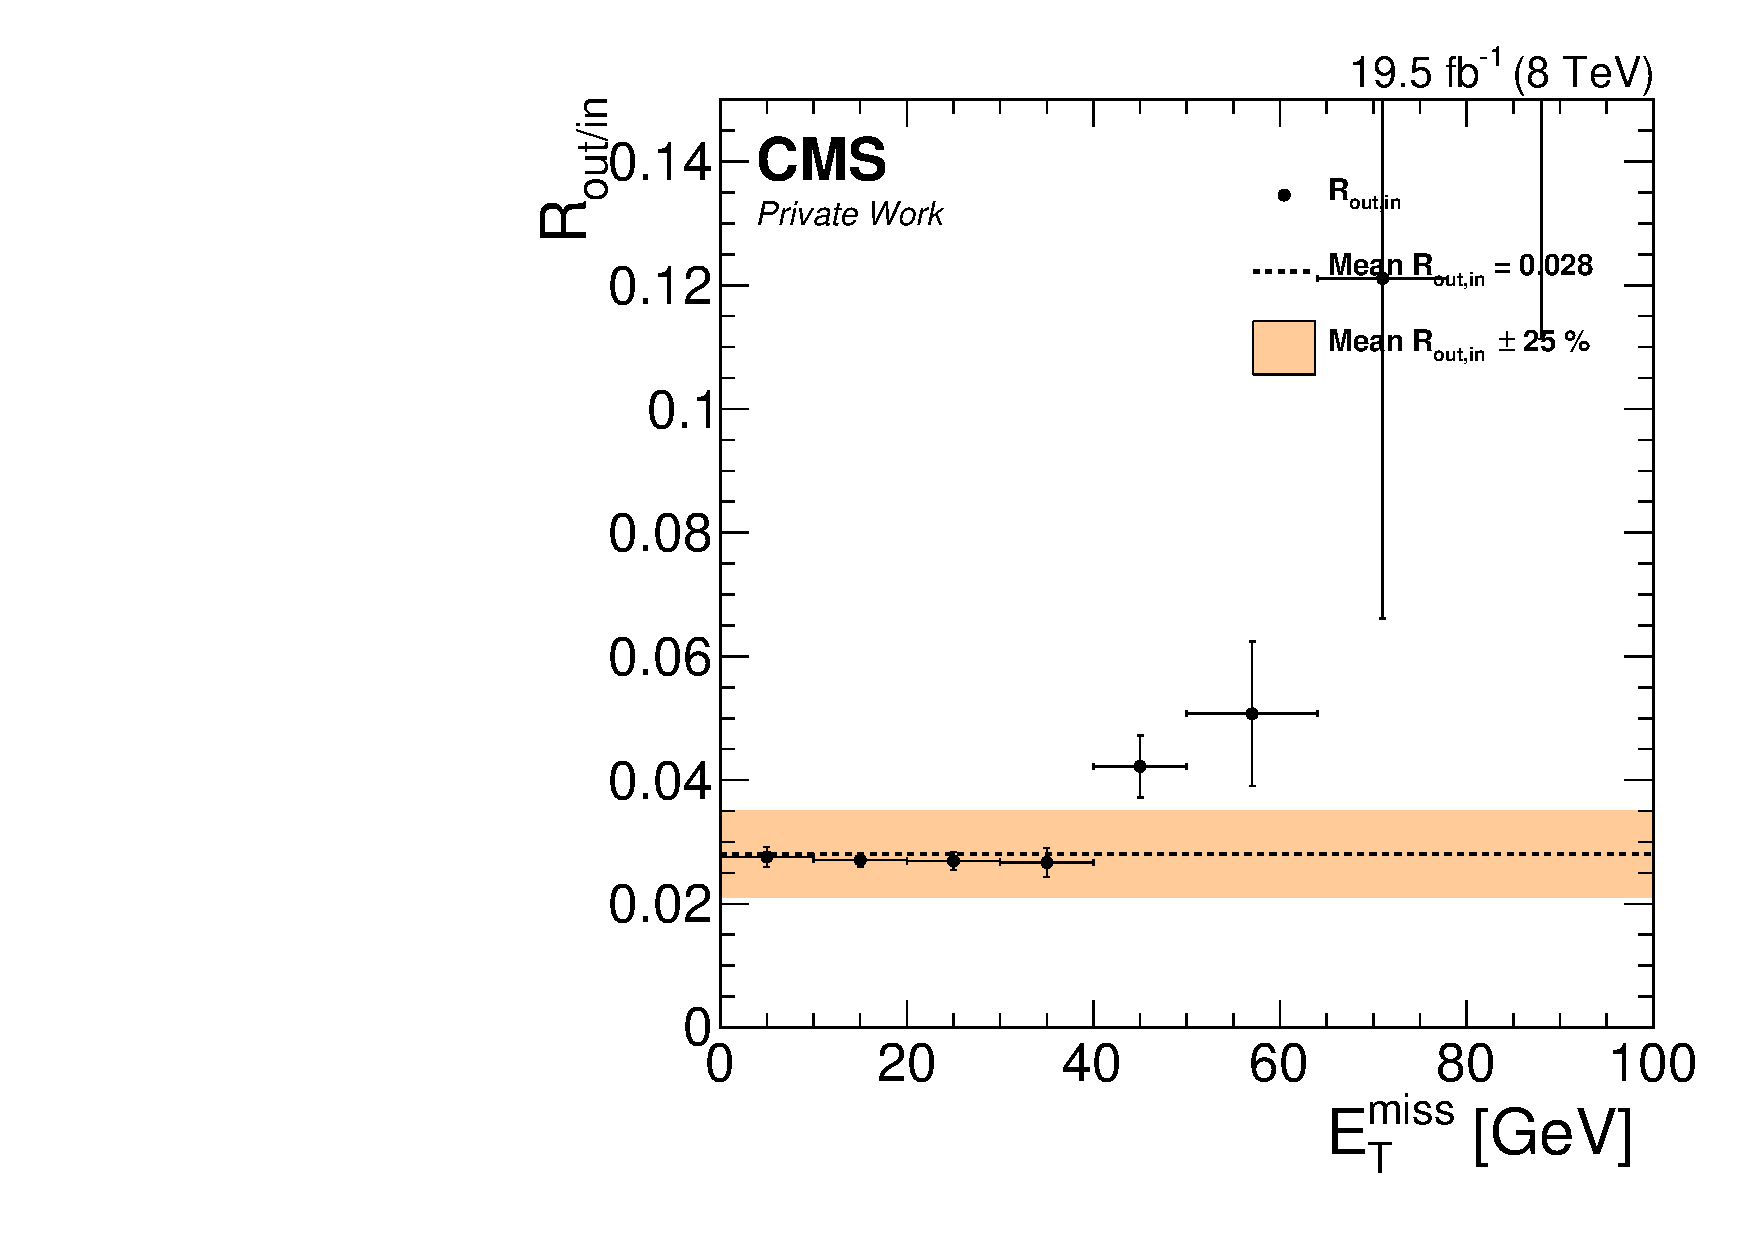
\includegraphics[width=\textwidth]{plots/BG/rOutIn/rOutInSyst_DrellYanControlForward_Full2012_MET_HighMass_SF_None.pdf}
\end{minipage}
\begin{minipage}[t]{0.49\textwidth}
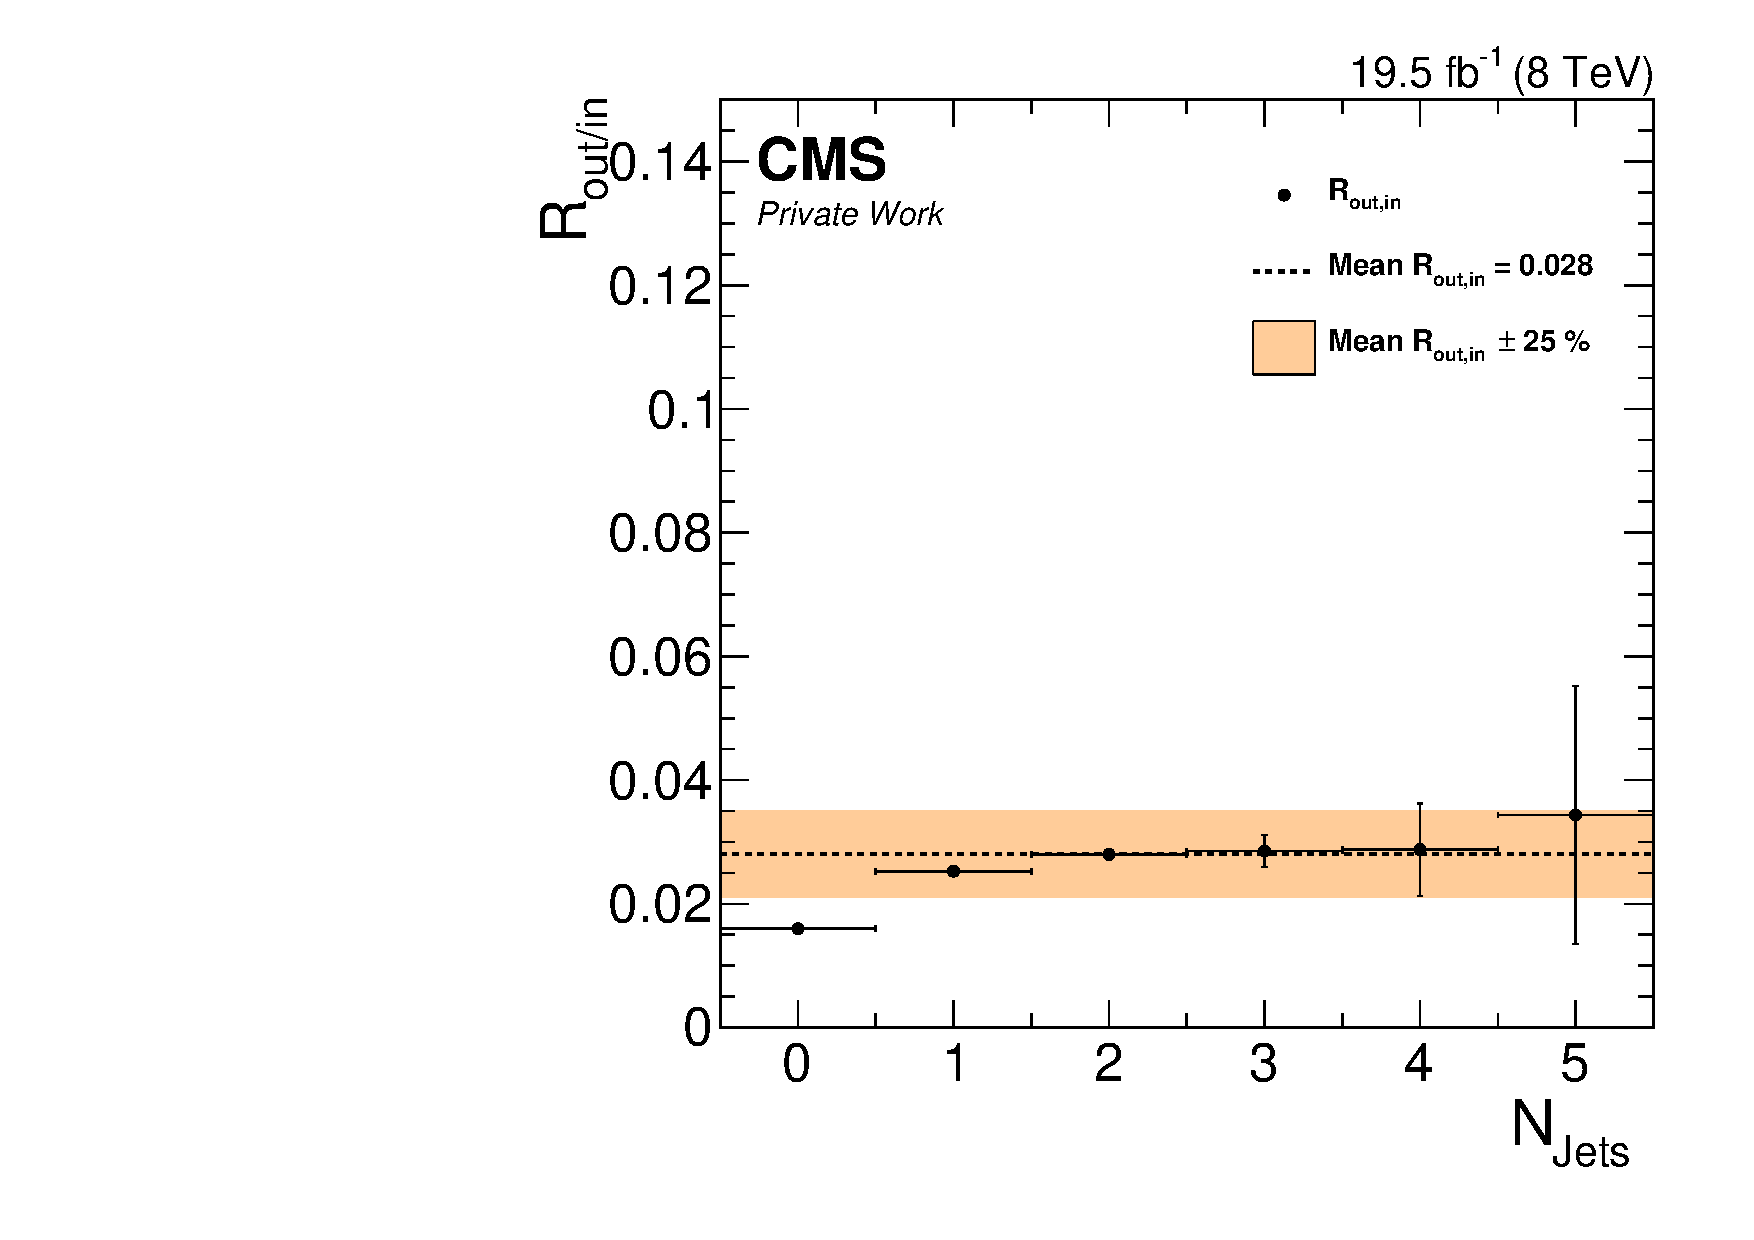
\includegraphics[width=\textwidth]{plots/BG/rOutIn/rOutInSyst_DrellYanControlForward_Full2012_NJets_HighMass_SF_None.pdf}
\end{minipage}
\caption{Dependencies of \Routin for the high-mass region on \MET (left) and \njets (right) for the central (top) and forward (bottom) lepton selection for SF lepton pairs. The results on data are shown in black. The central value is shown as a black dashed line while the systematic uncertainty is shown as an orange band.}
\label{fig:ROutInDependencies2}
\end{figure} 



\begin{figure}[htbp]
\centering
\begin{minipage}[t]{0.49\textwidth}
  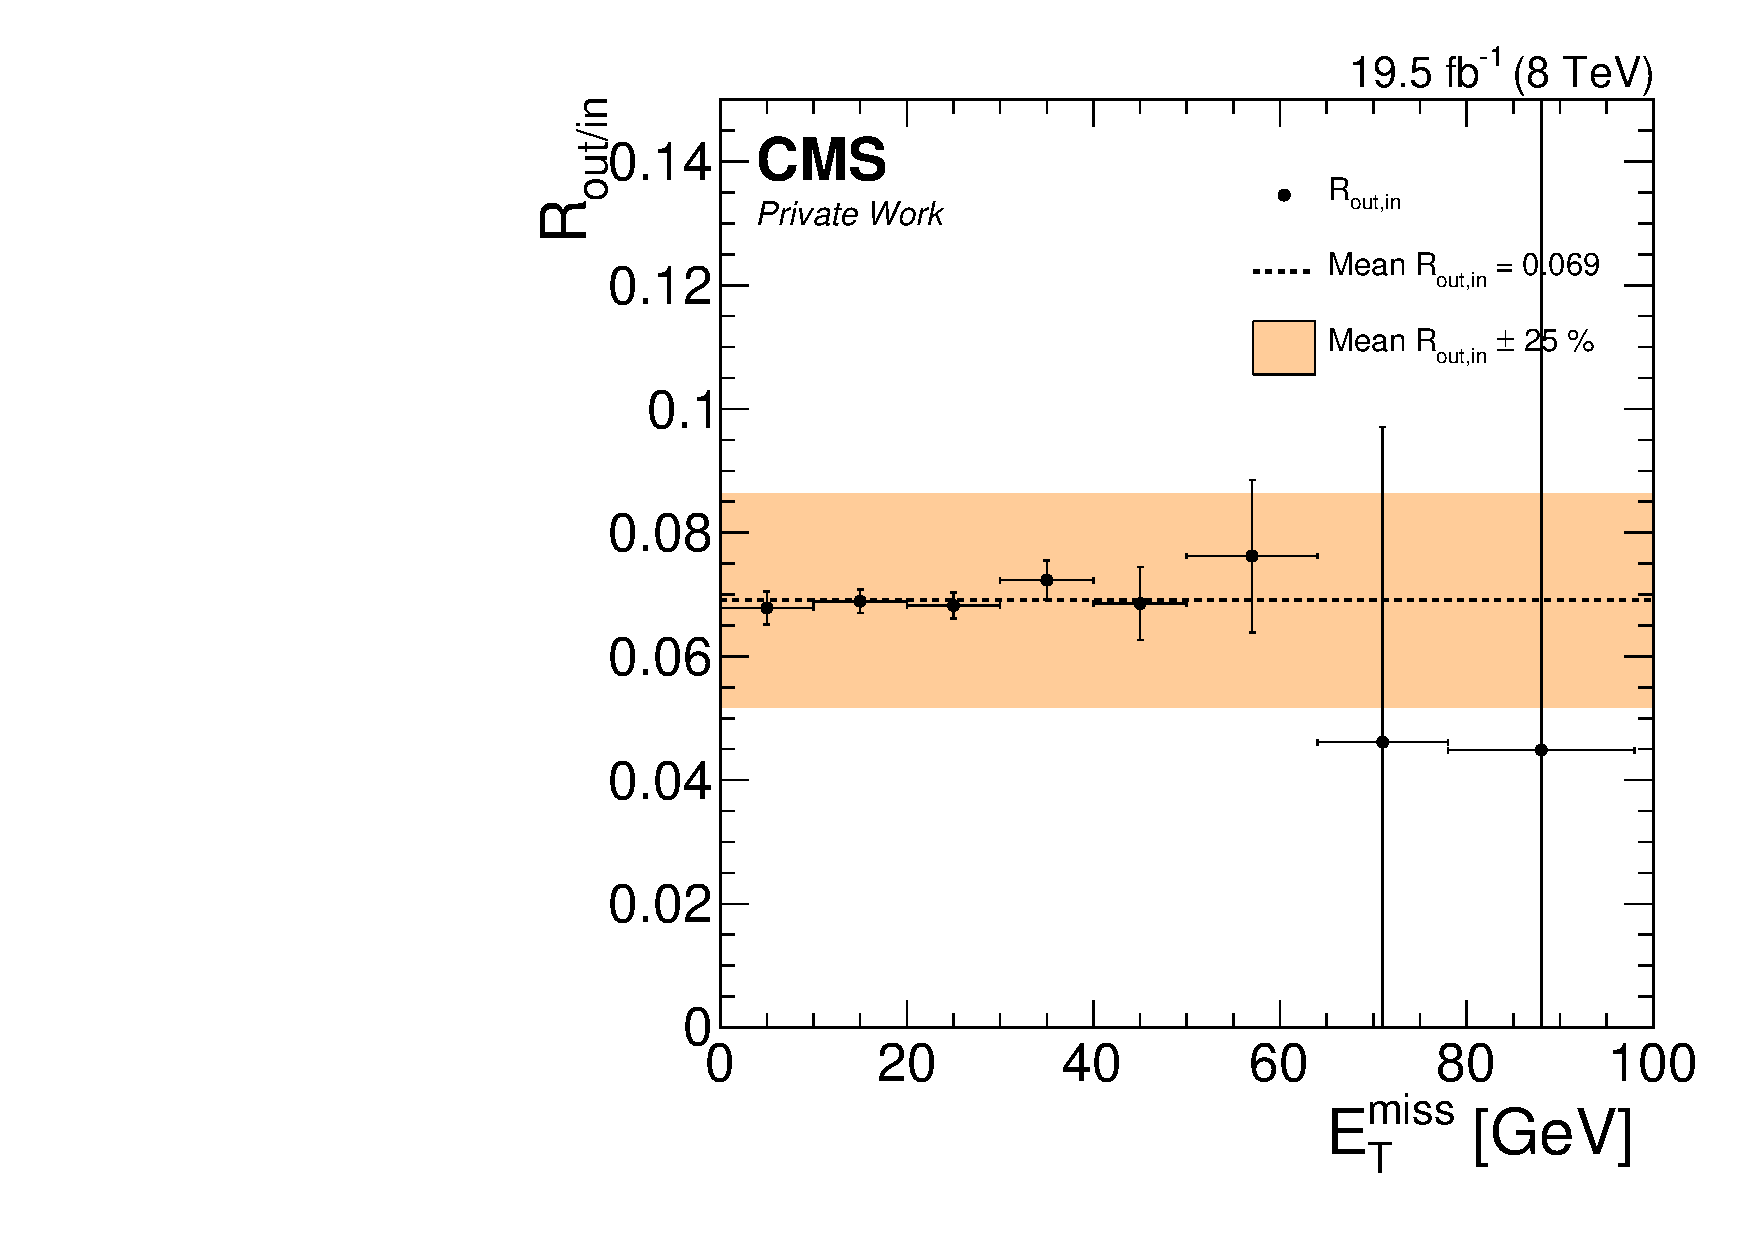
\includegraphics[width=\textwidth]{plots/BG/rOutIn/rOutInSyst_DrellYanControlCentral_Full2012_MET_LowMass_EE_None.pdf}
\end{minipage}
\begin{minipage}[t]{0.49\textwidth}
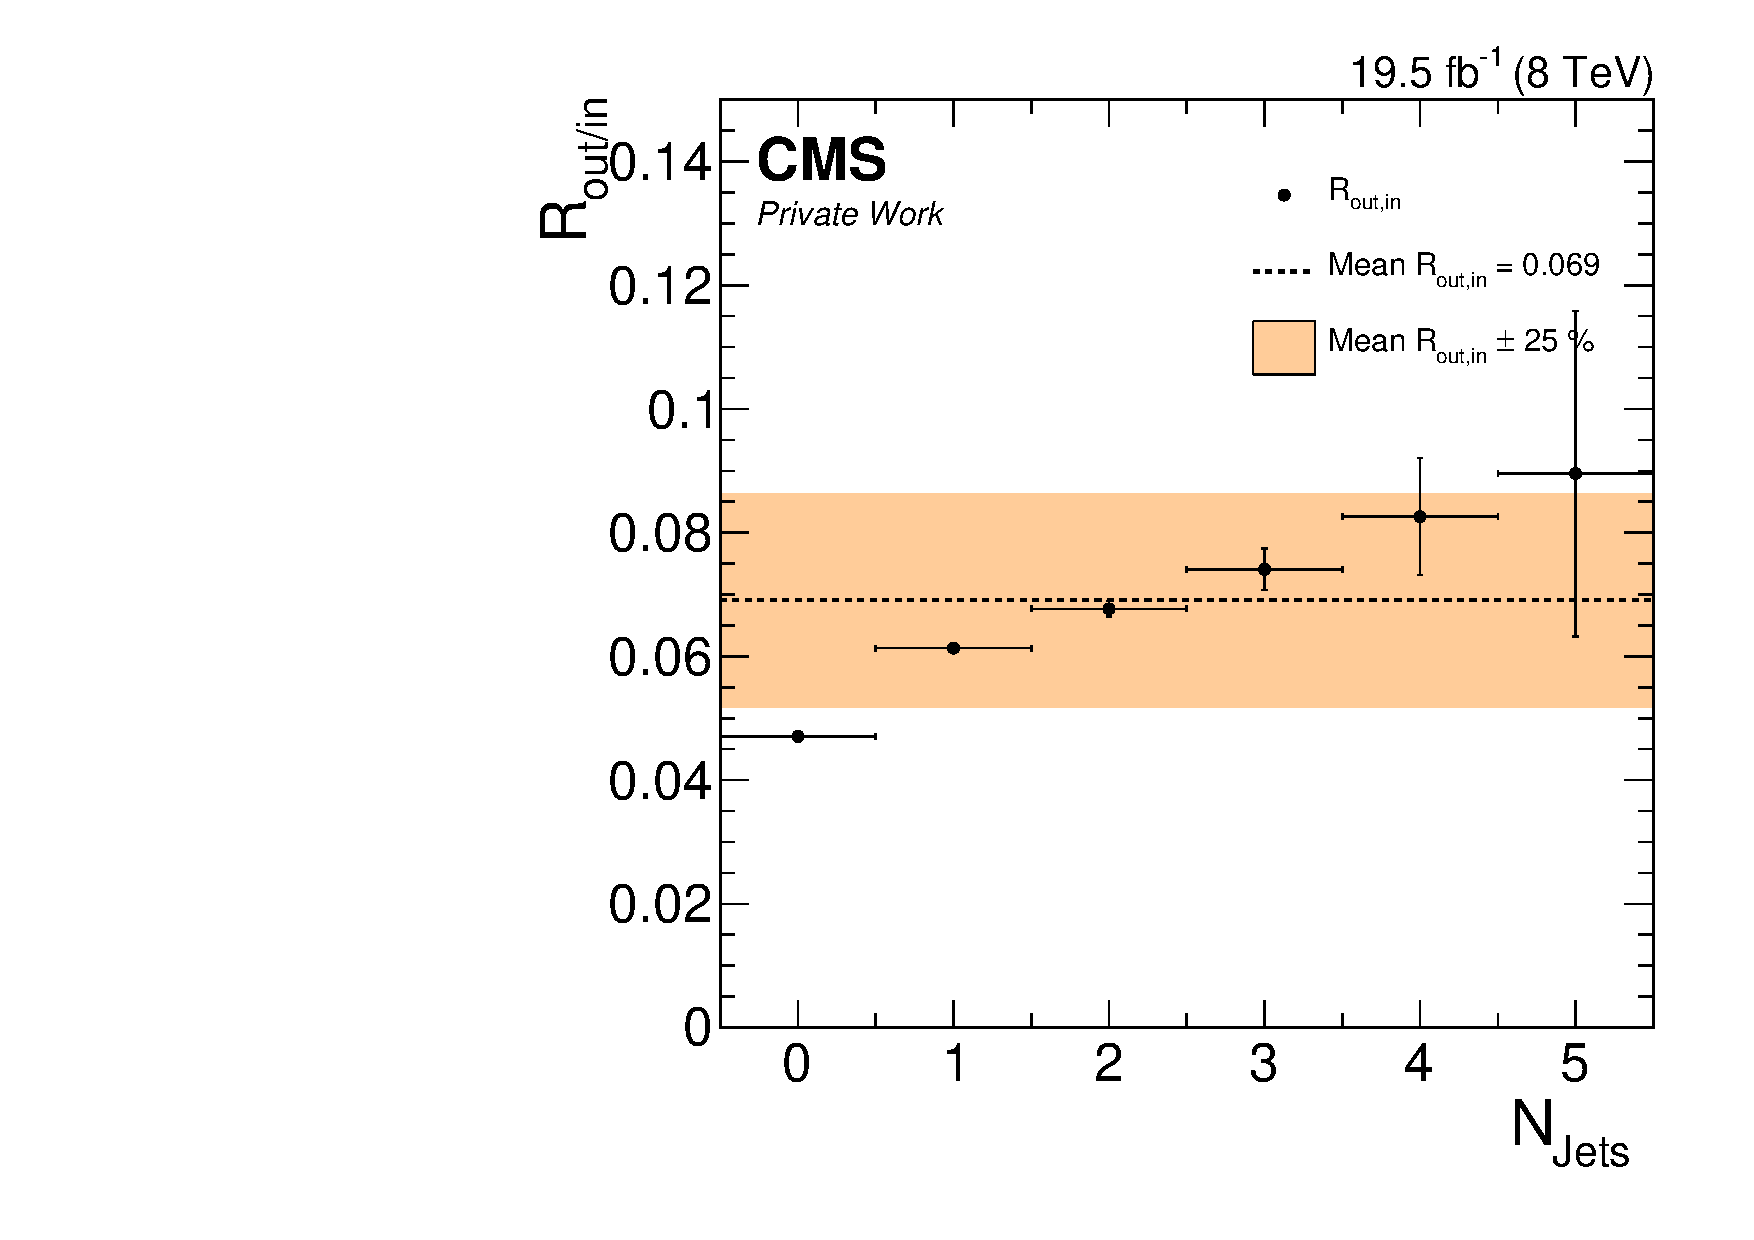
\includegraphics[width=\textwidth]{plots/BG/rOutIn/rOutInSyst_DrellYanControlCentral_Full2012_NJets_LowMass_EE_None.pdf}
\end{minipage}
\begin{minipage}[t]{0.49\textwidth}
  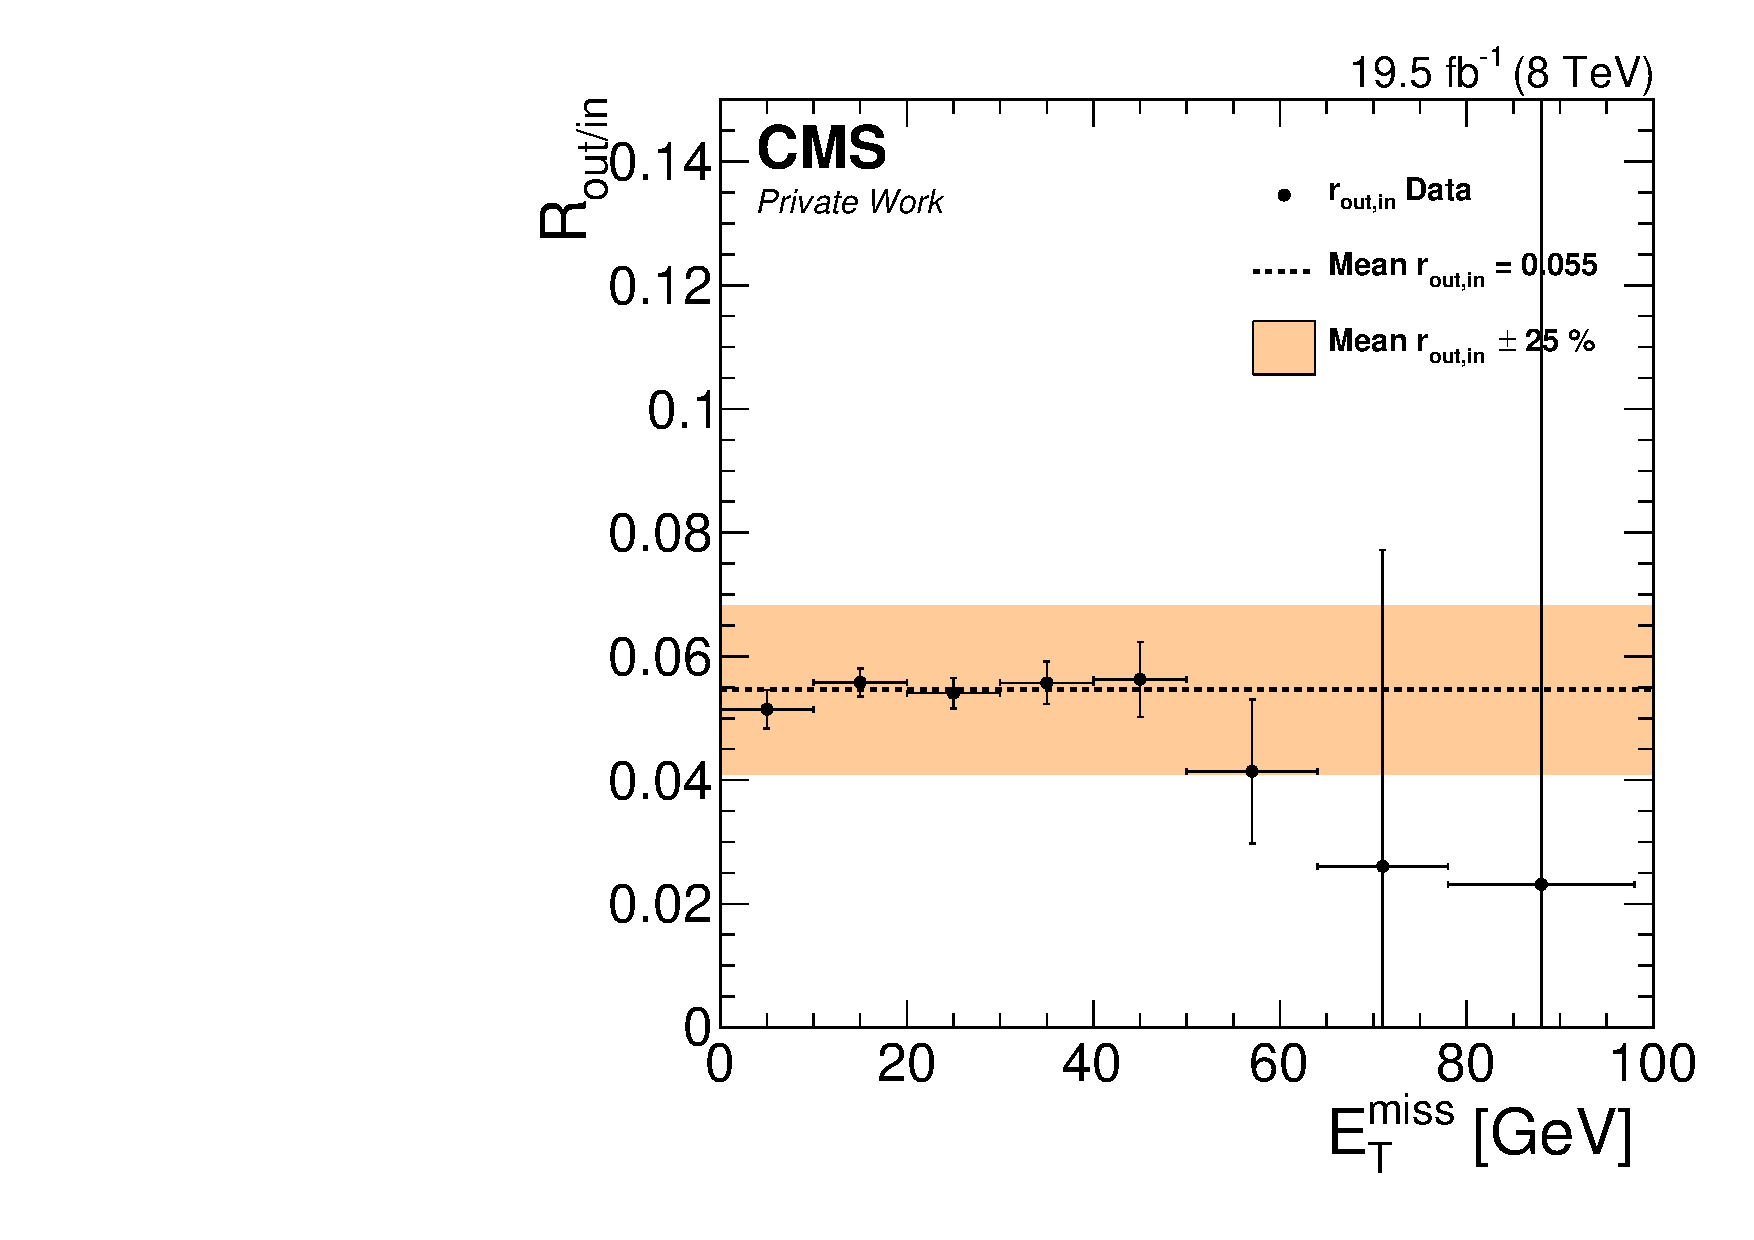
\includegraphics[width=\textwidth]{plots/BG/rOutIn/rOutInSyst_DrellYanControlForward_Full2012_MET_LowMass_EE_None.pdf}
\end{minipage}
\begin{minipage}[t]{0.49\textwidth}
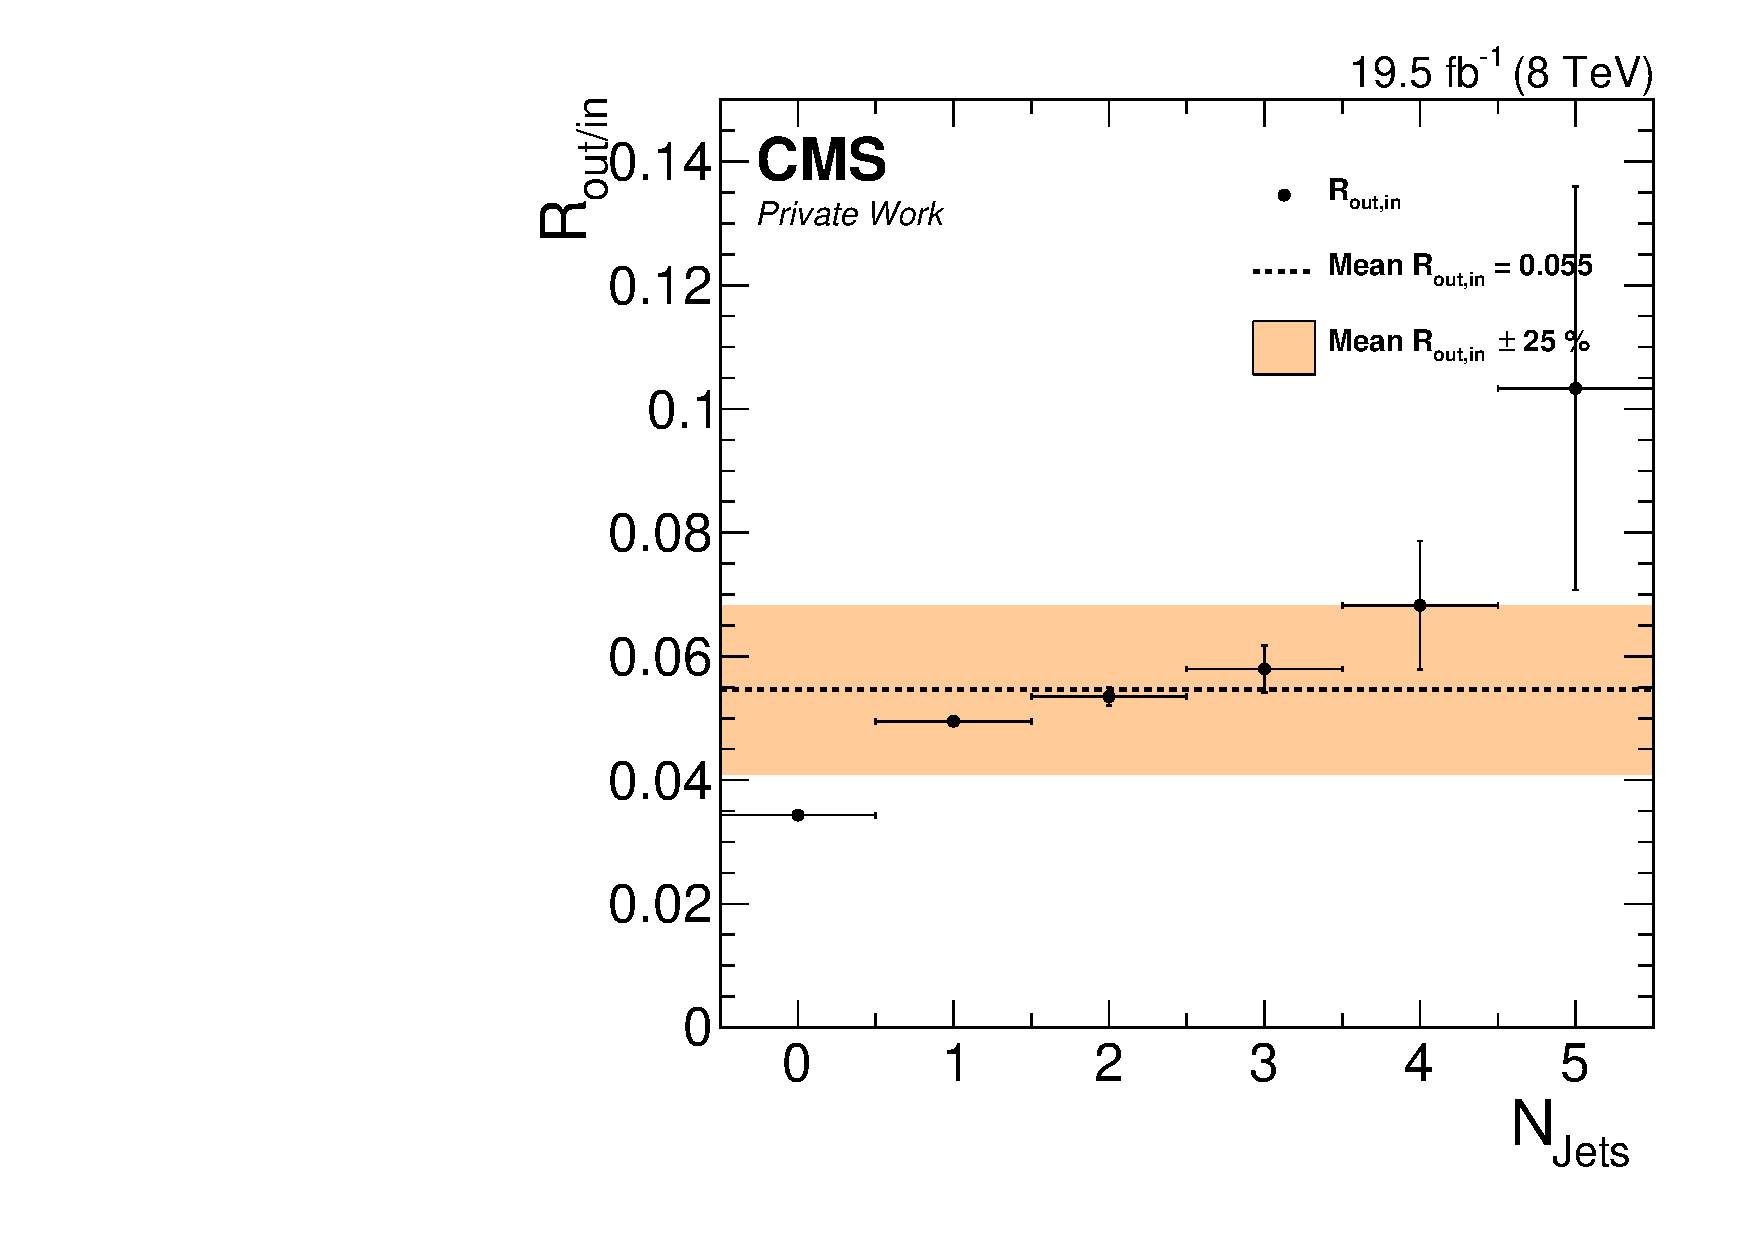
\includegraphics[width=\textwidth]{plots/BG/rOutIn/rOutInSyst_DrellYanControlForward_Full2012_NJets_LowMass_EE_None.pdf}
\end{minipage}
\caption{Dependencies of \Routin for the low-mass region on \MET (left) and \njets (right) for the central (top) and forward (bottom) lepton selection for \EE lepton pairs. The results on data are shown in black. The central value is shown as a black dashed line while the systematic uncertainty is shown as an orange band.}
\label{fig:ROutInDependencies3}
\end{figure} 


\begin{figure}[htbp]
\centering
\begin{minipage}[t]{0.49\textwidth}
  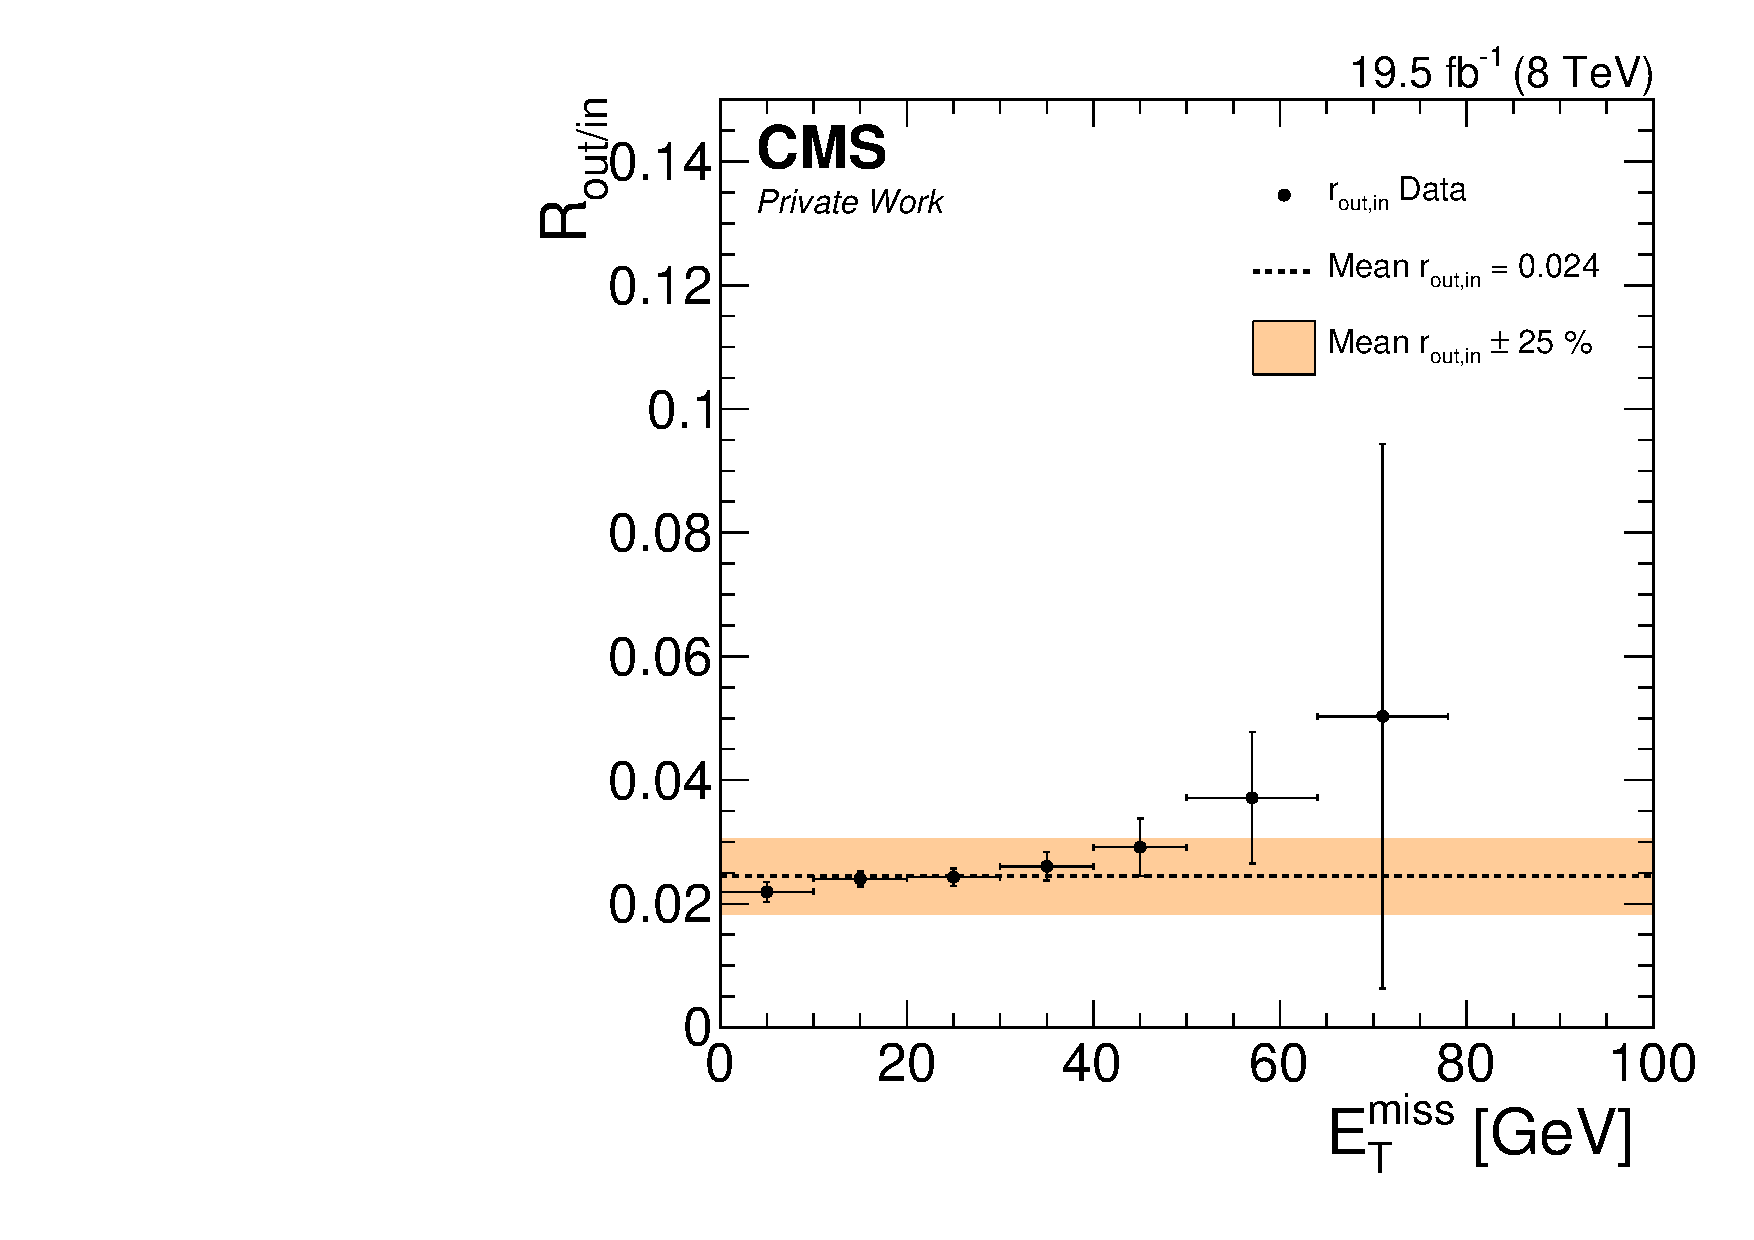
\includegraphics[width=\textwidth]{plots/BG/rOutIn/rOutInSyst_DrellYanControlCentral_Full2012_MET_HighMass_EE_None.pdf}
\end{minipage}
\begin{minipage}[t]{0.49\textwidth}
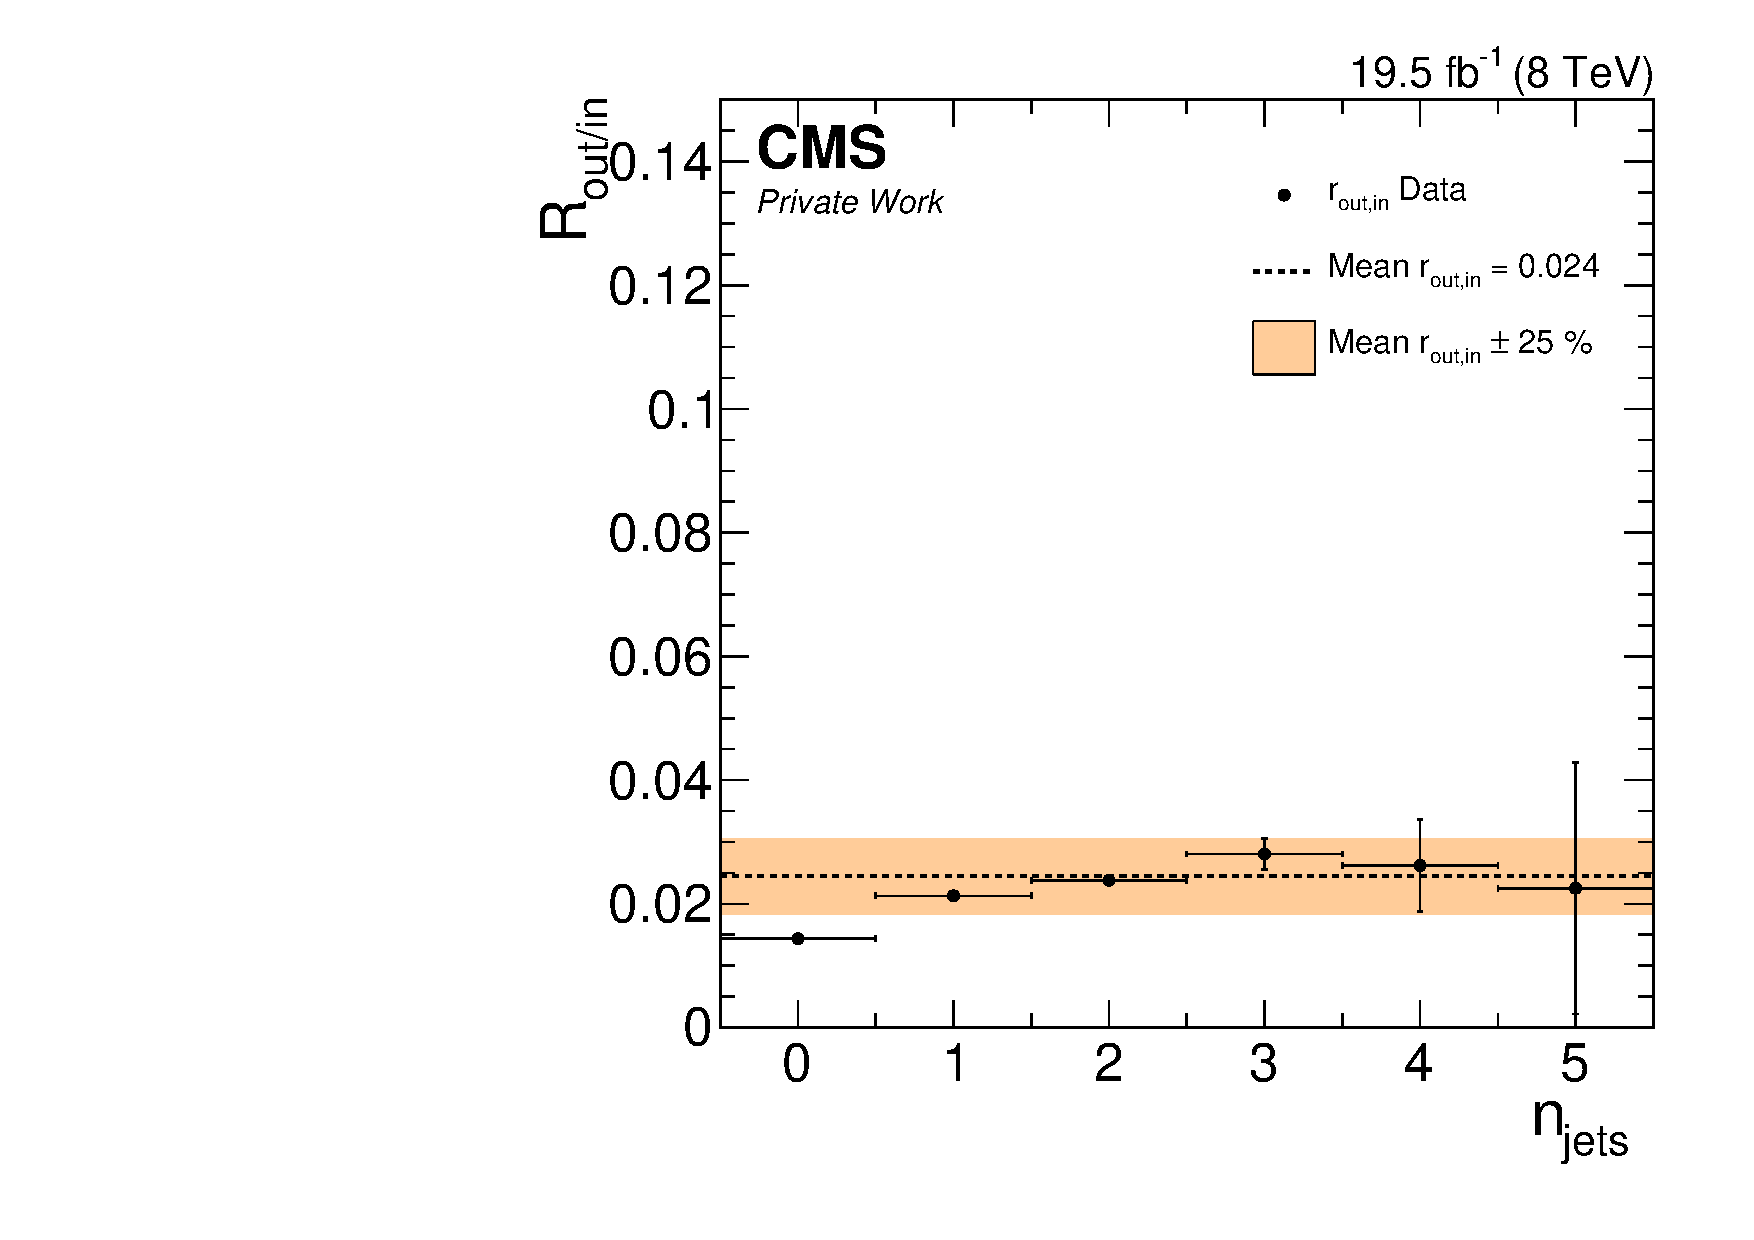
\includegraphics[width=\textwidth]{plots/BG/rOutIn/rOutInSyst_DrellYanControlCentral_Full2012_NJets_HighMass_EE_None.pdf}
\end{minipage}
\begin{minipage}[t]{0.49\textwidth}
  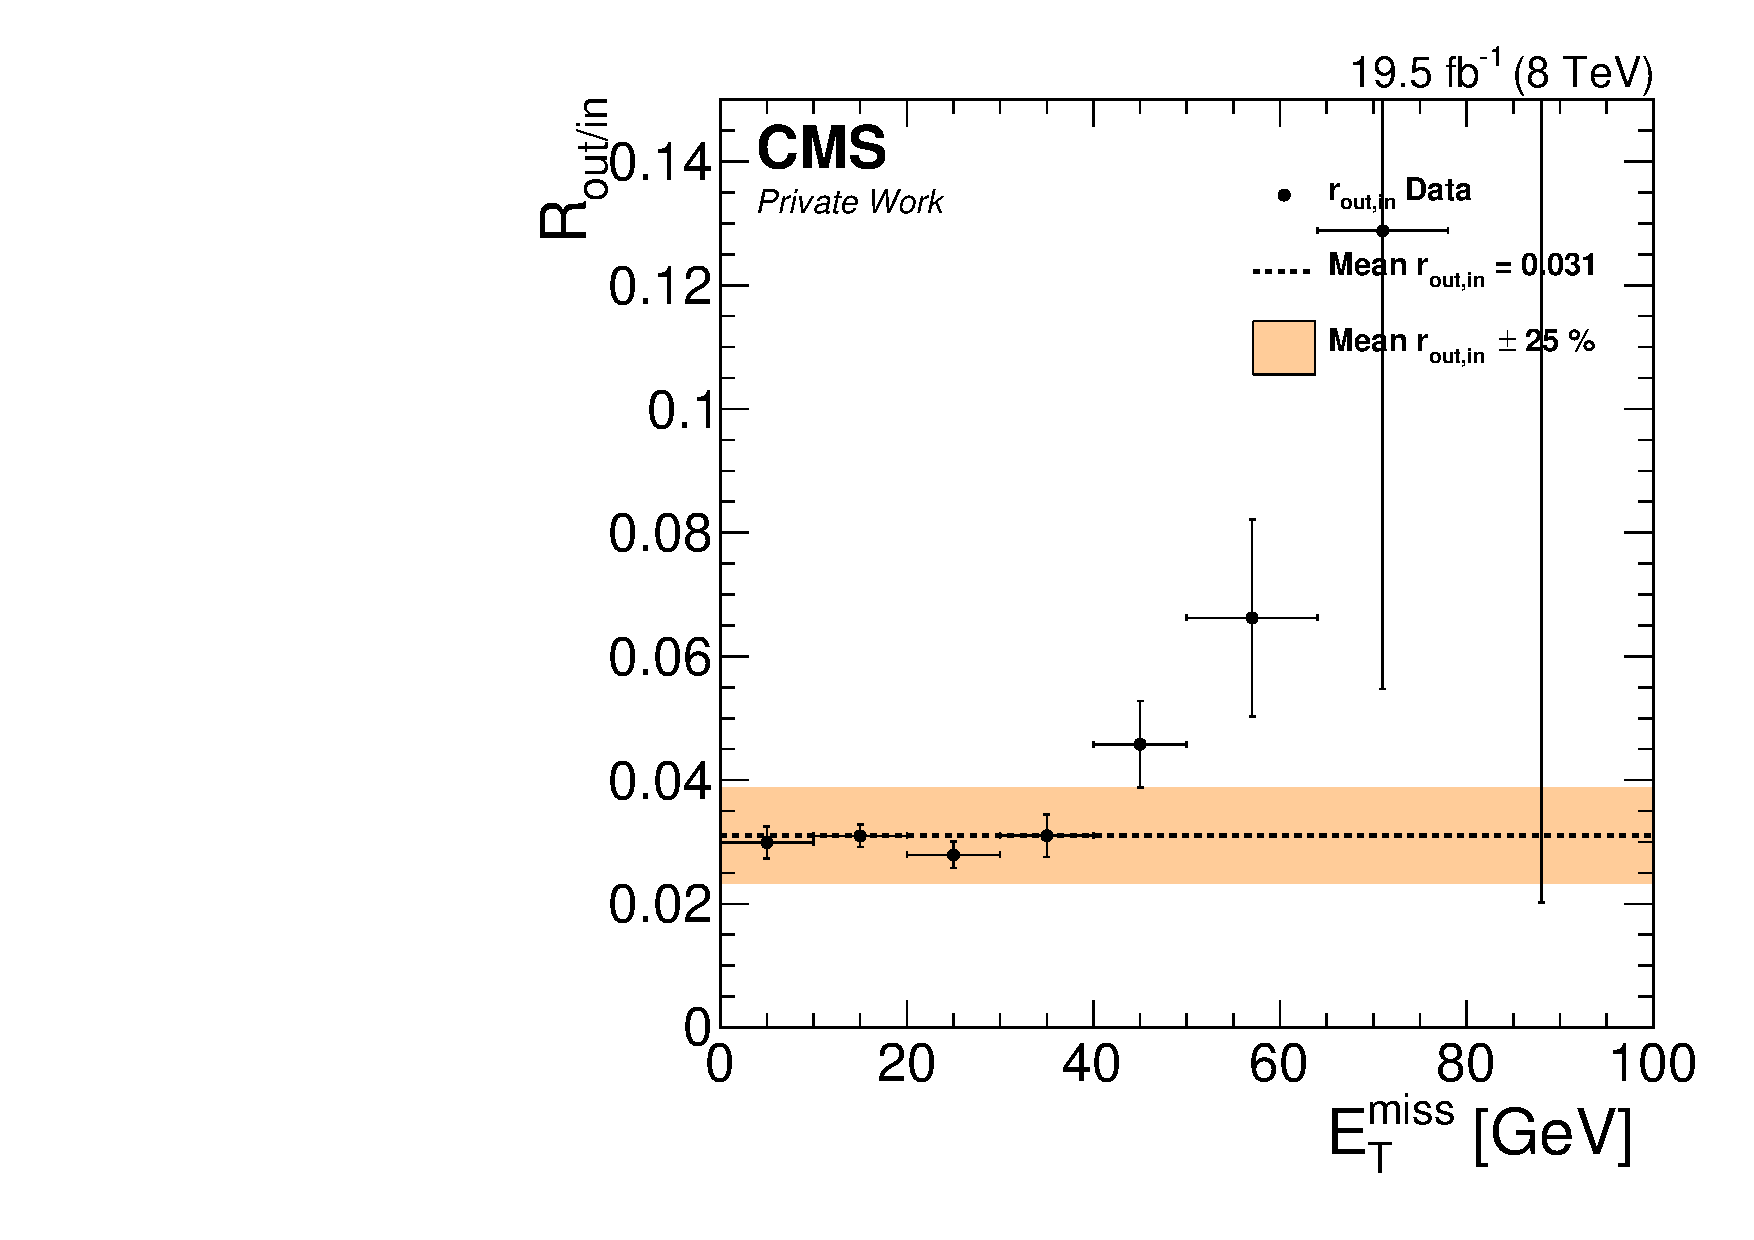
\includegraphics[width=\textwidth]{plots/BG/rOutIn/rOutInSyst_DrellYanControlForward_Full2012_MET_HighMass_EE_None.pdf}
\end{minipage}
\begin{minipage}[t]{0.49\textwidth}
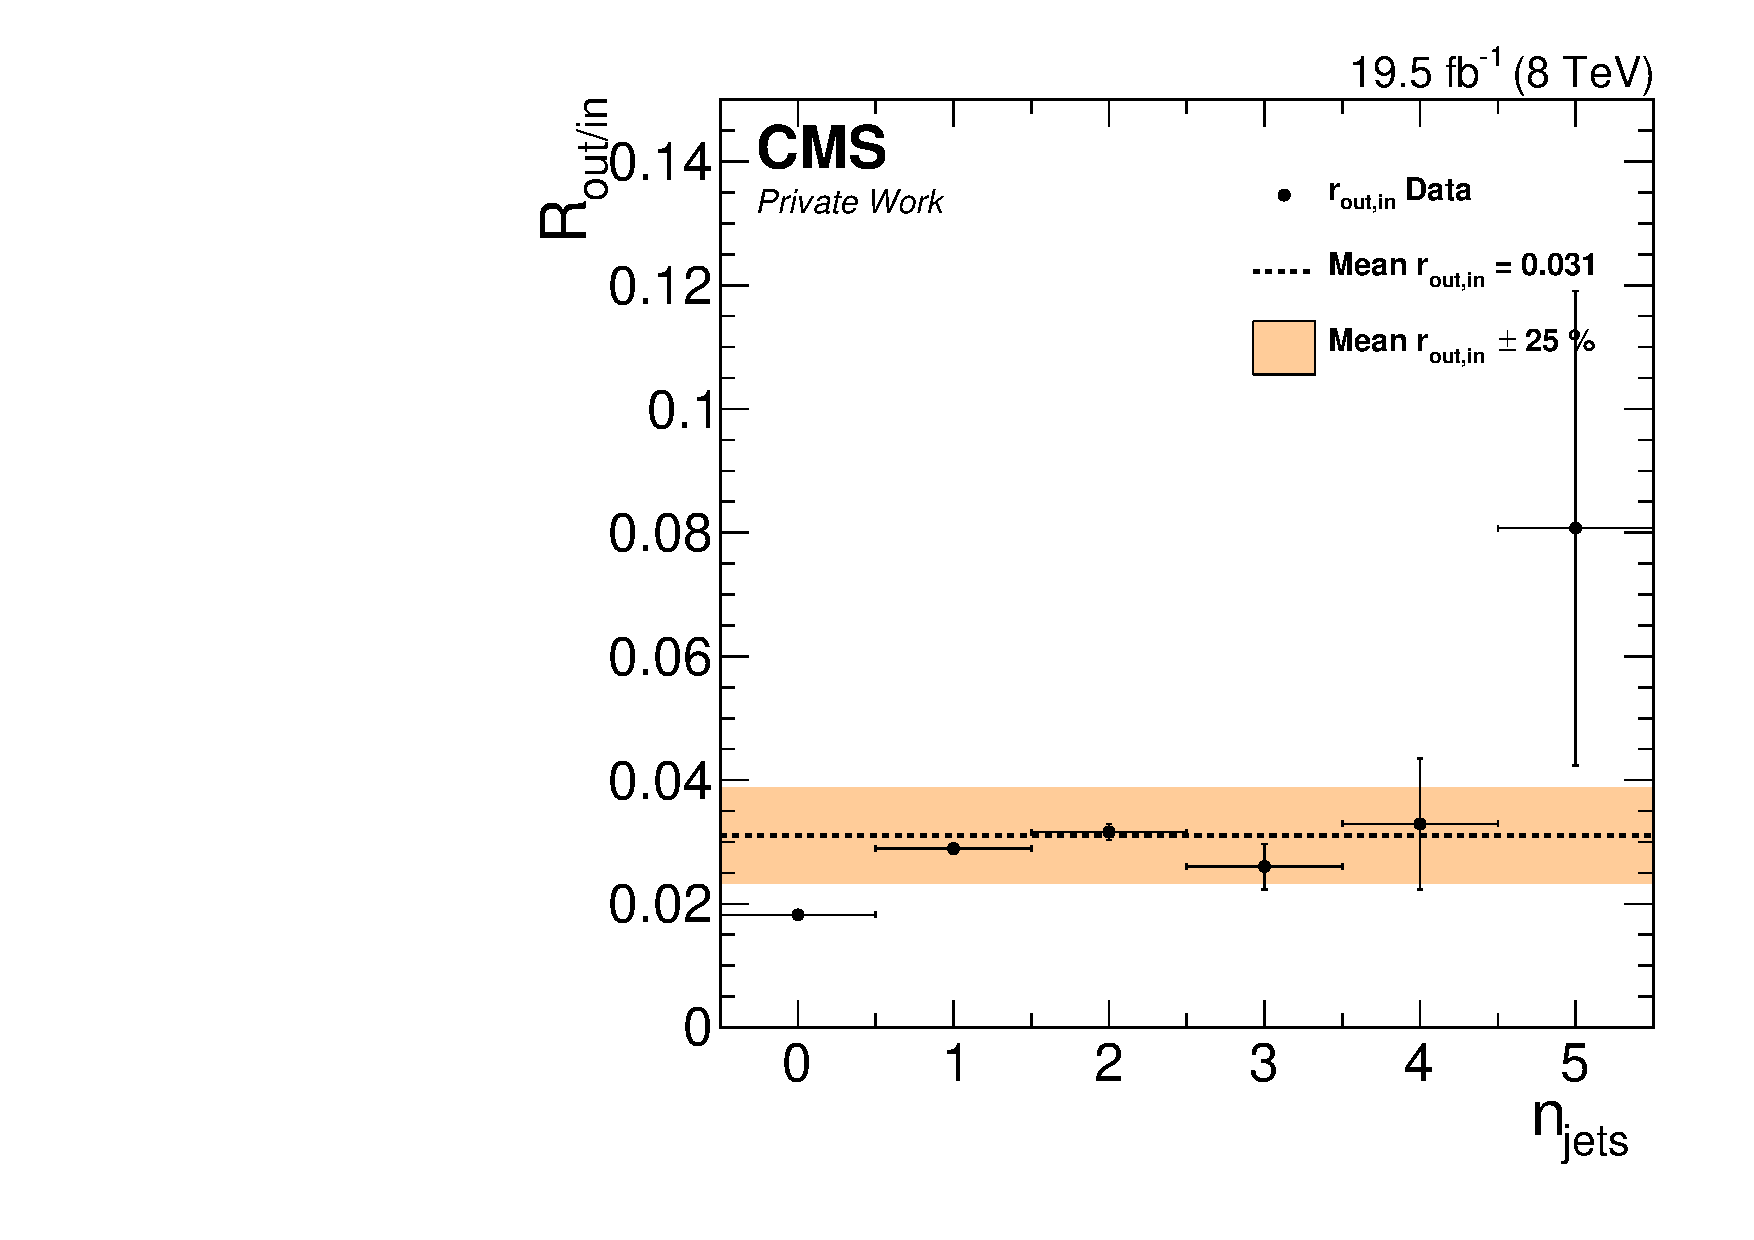
\includegraphics[width=\textwidth]{plots/BG/rOutIn/rOutInSyst_DrellYanControlForward_Full2012_NJets_HighMass_EE_None.pdf}
\end{minipage}
\caption{Dependencies of \Routin for the high-mass region on \MET (left) and \njets (right) for the central (top) and forward (bottom) lepton selection for \EE lepton pairs. The results on data are shown in black. The central value is shown as a black dashed line while the systematic uncertainty is shown as an orange band.}
\label{fig:ROutInDependencies4}
\end{figure} 

\begin{figure}[htbp]
\centering
\begin{minipage}[t]{0.49\textwidth}
  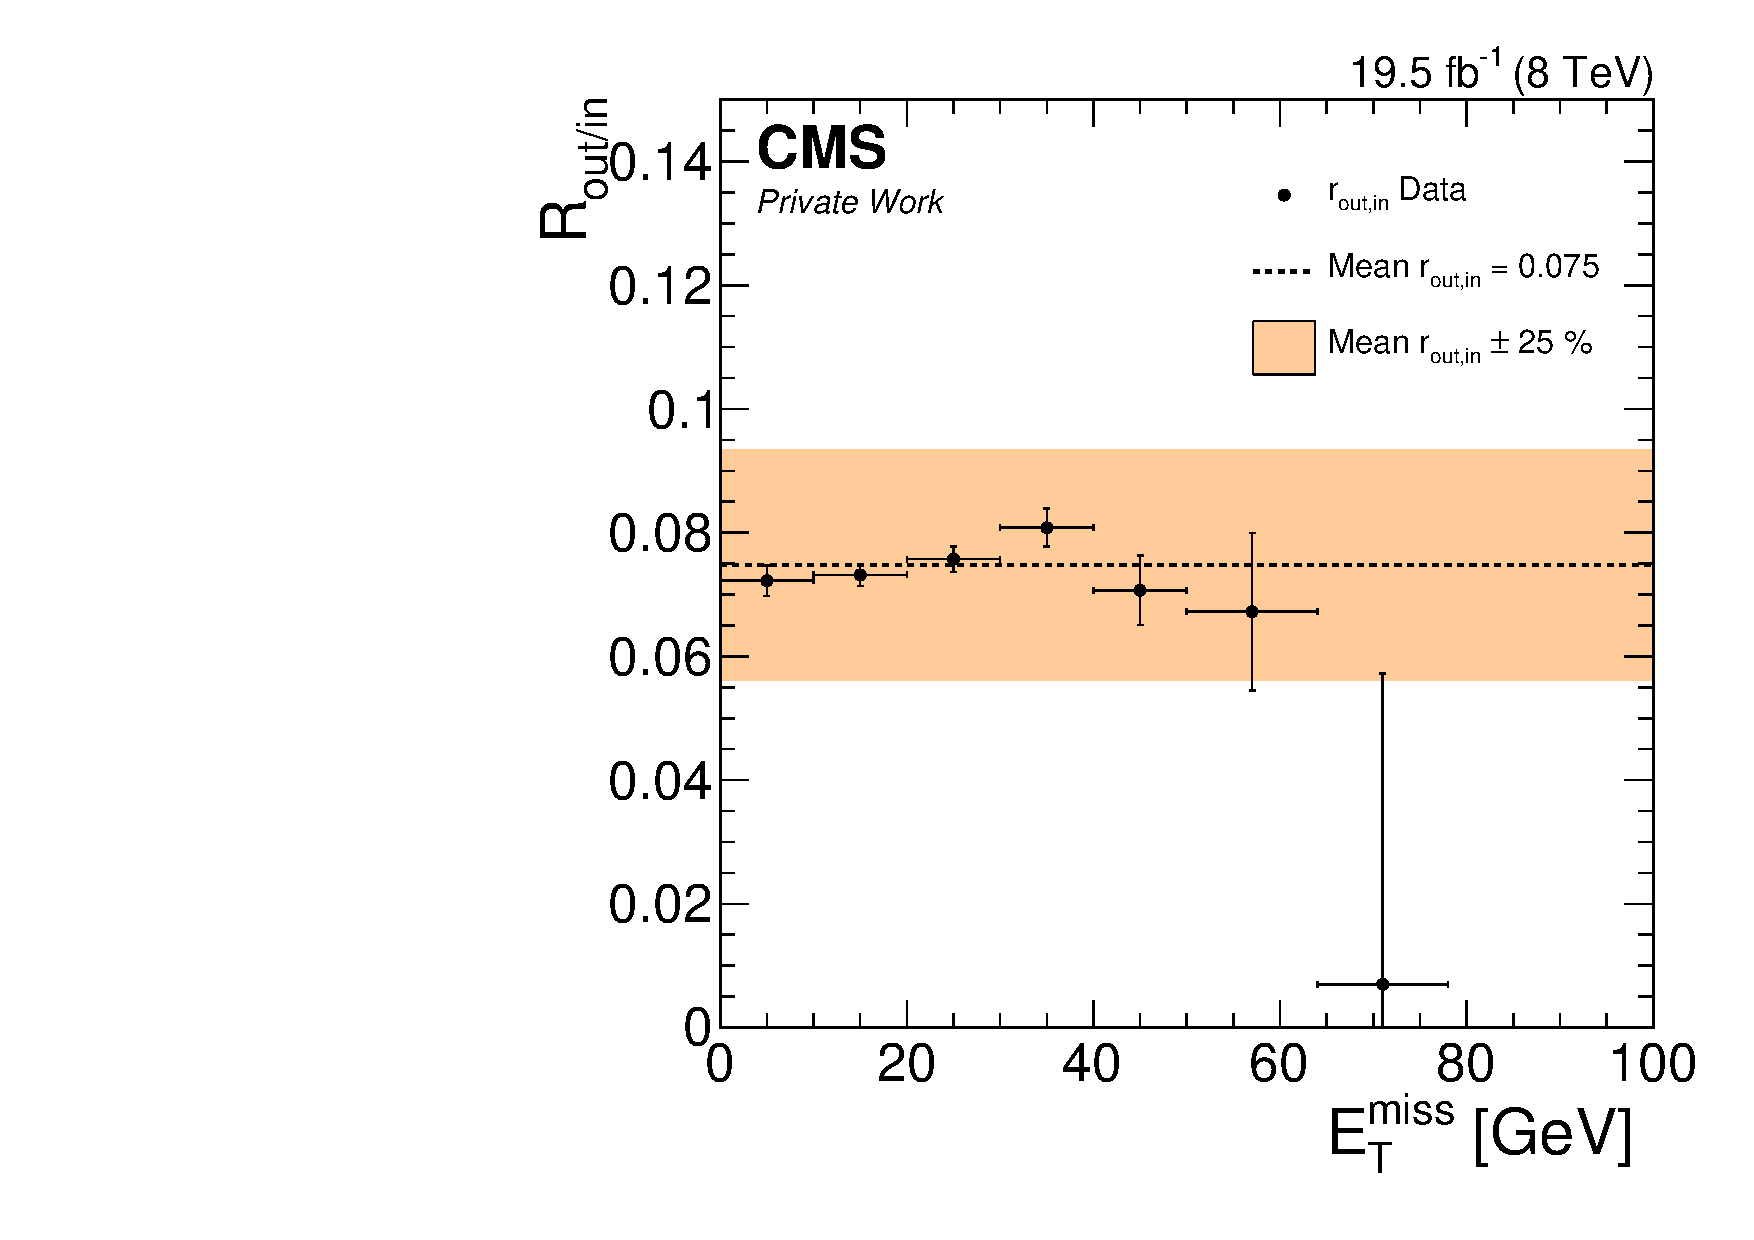
\includegraphics[width=\textwidth]{plots/BG/rOutIn/rOutInSyst_DrellYanControlCentral_Full2012_MET_LowMass_MM_None.pdf}
\end{minipage}
\begin{minipage}[t]{0.49\textwidth}
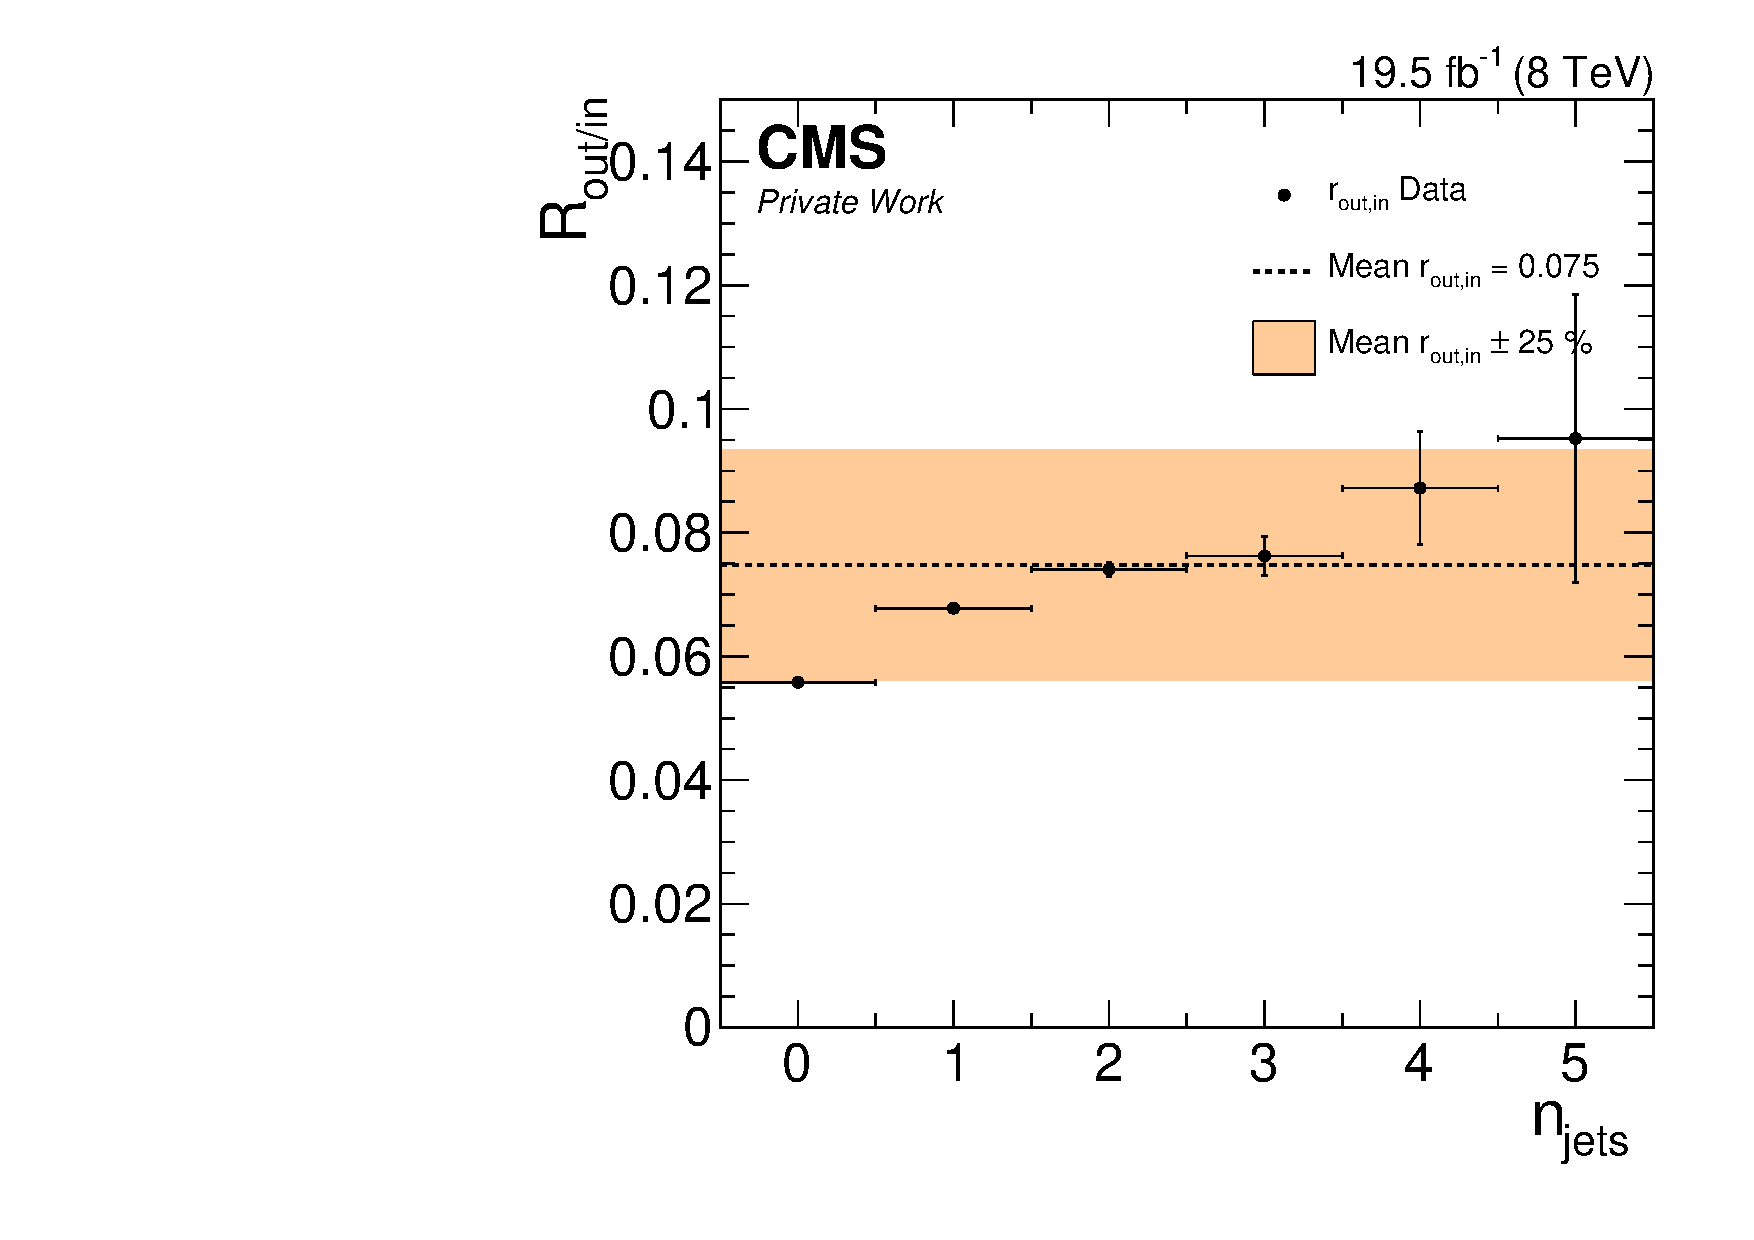
\includegraphics[width=\textwidth]{plots/BG/rOutIn/rOutInSyst_DrellYanControlCentral_Full2012_NJets_LowMass_MM_None.pdf}
\end{minipage}
\begin{minipage}[t]{0.49\textwidth}
  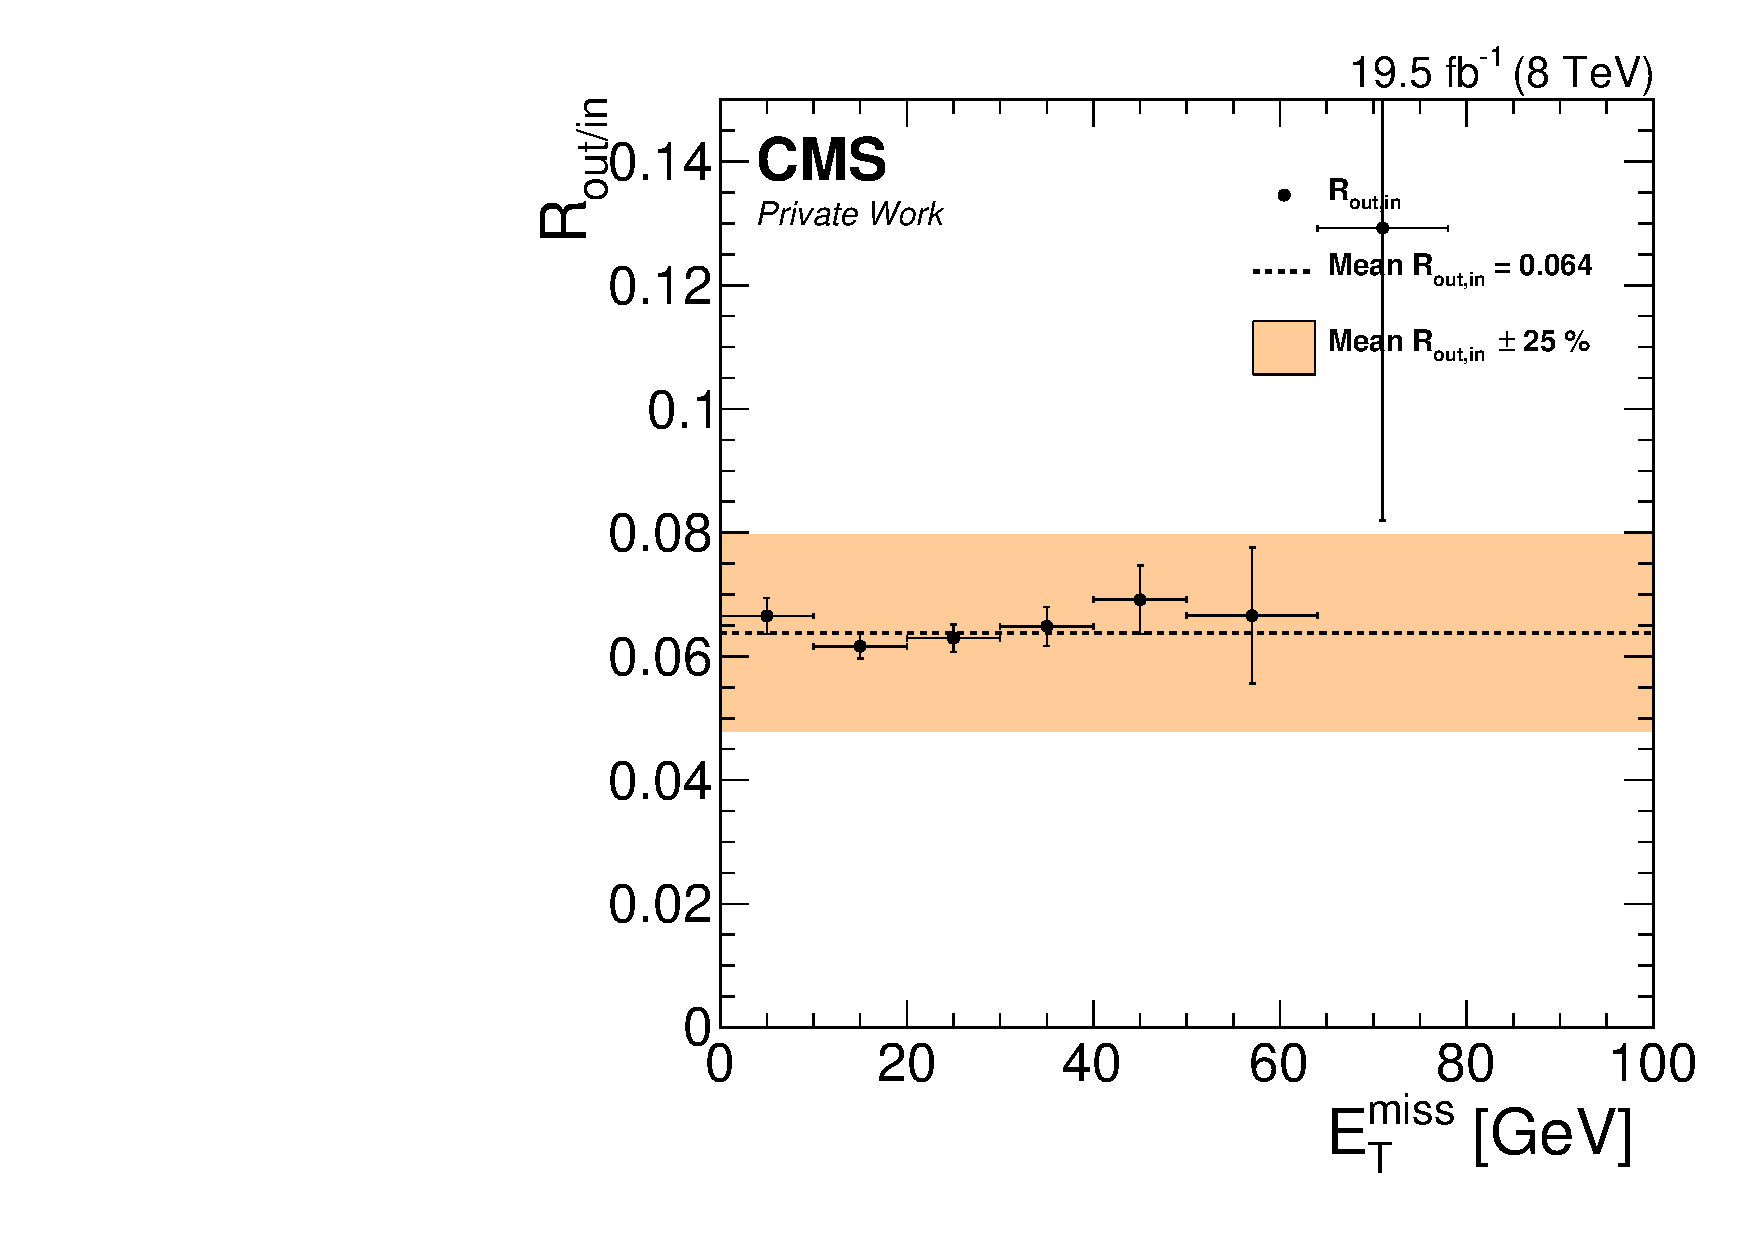
\includegraphics[width=\textwidth]{plots/BG/rOutIn/rOutInSyst_DrellYanControlForward_Full2012_MET_LowMass_MM_None.pdf}
\end{minipage}
\begin{minipage}[t]{0.49\textwidth}
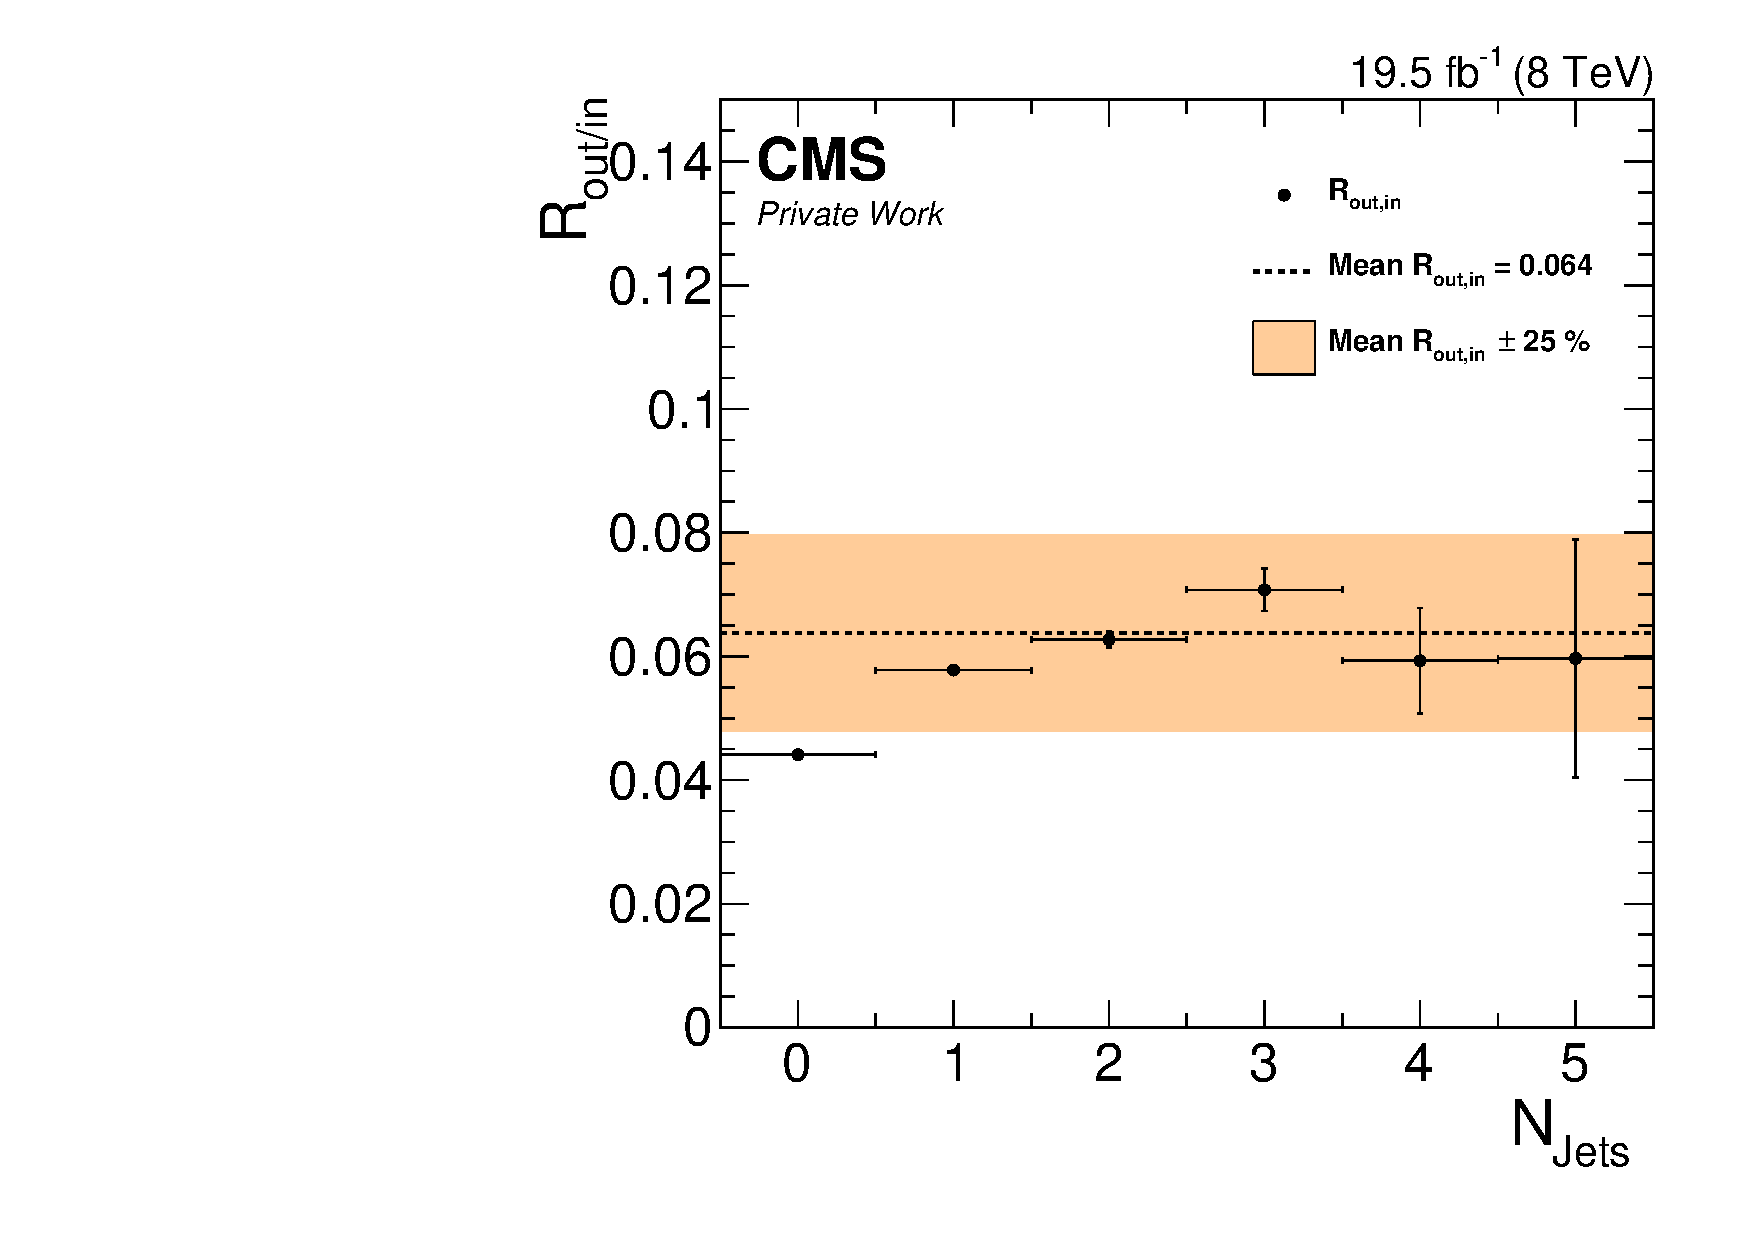
\includegraphics[width=\textwidth]{plots/BG/rOutIn/rOutInSyst_DrellYanControlForward_Full2012_NJets_LowMass_MM_None.pdf}
\end{minipage}
\caption{Dependencies of \Routin for the low-mass region on \MET (left) and \njets (right) for the central (top) and forward (bottom) lepton selection for \MM lepton pairs. The results on data are shown in black. The central value is shown as a black dashed line while the systematic uncertainty is shown as an orange band.}
\label{fig:ROutInDependencies5}
\end{figure} 


\begin{figure}[htbp]
\centering
\begin{minipage}[t]{0.49\textwidth}
  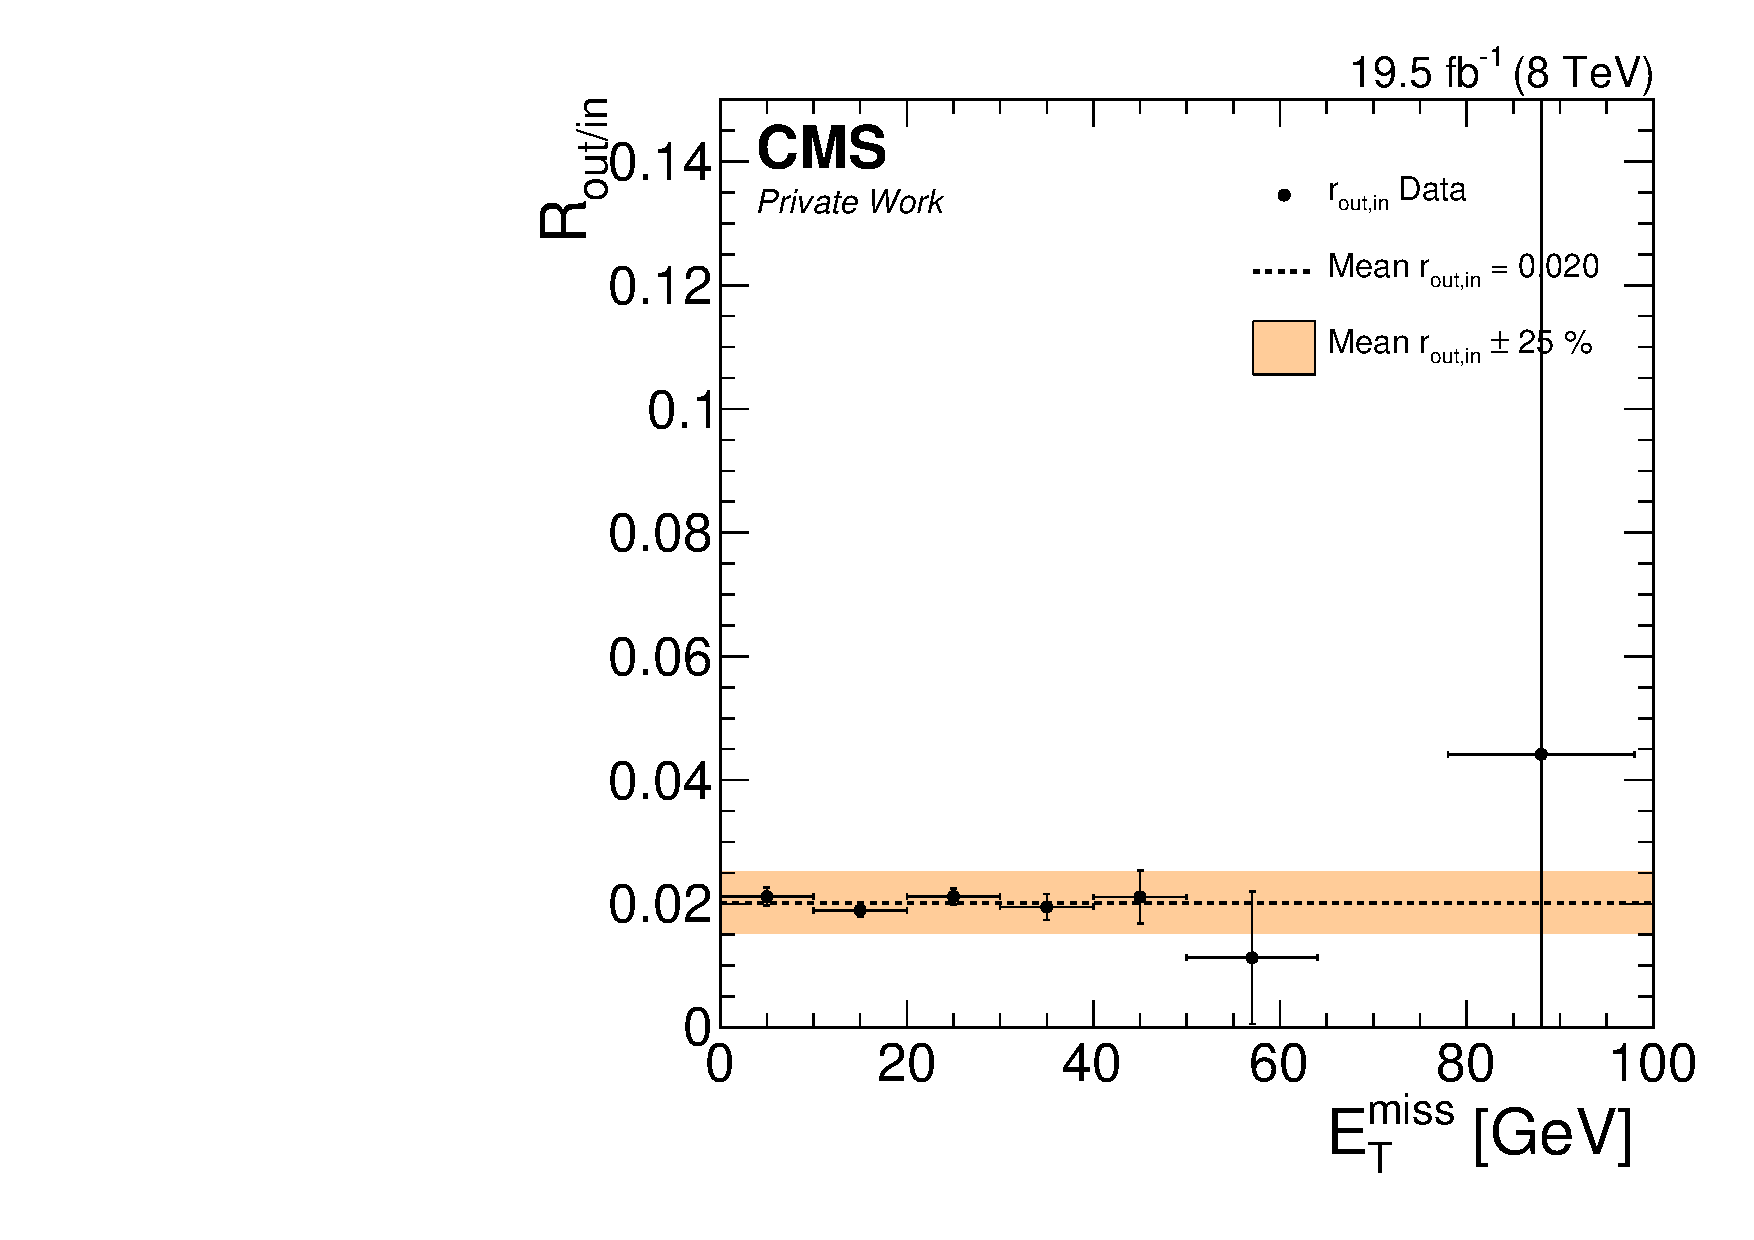
\includegraphics[width=\textwidth]{plots/BG/rOutIn/rOutInSyst_DrellYanControlCentral_Full2012_MET_HighMass_MM_None.pdf}
\end{minipage}
\begin{minipage}[t]{0.49\textwidth}
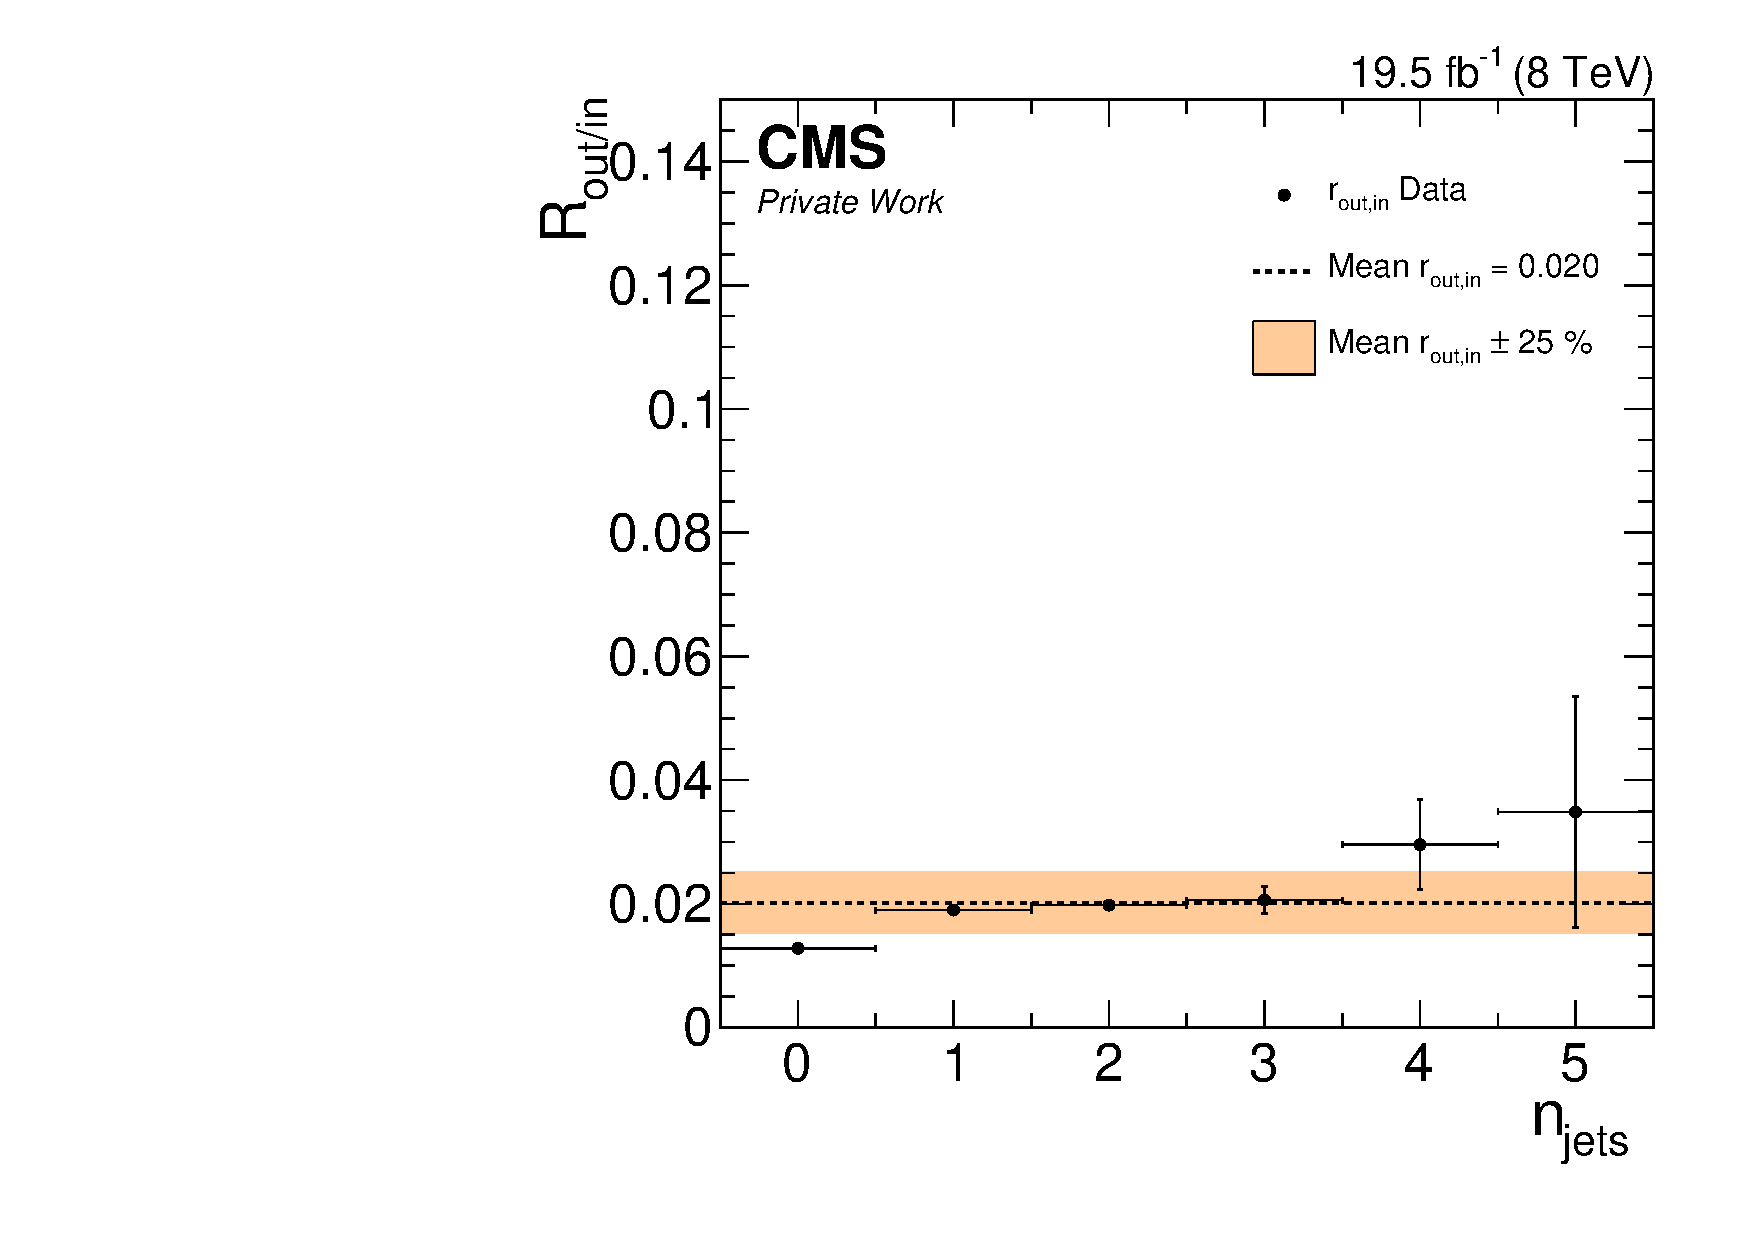
\includegraphics[width=\textwidth]{plots/BG/rOutIn/rOutInSyst_DrellYanControlCentral_Full2012_NJets_HighMass_MM_None.pdf}
\end{minipage}
\begin{minipage}[t]{0.49\textwidth}
  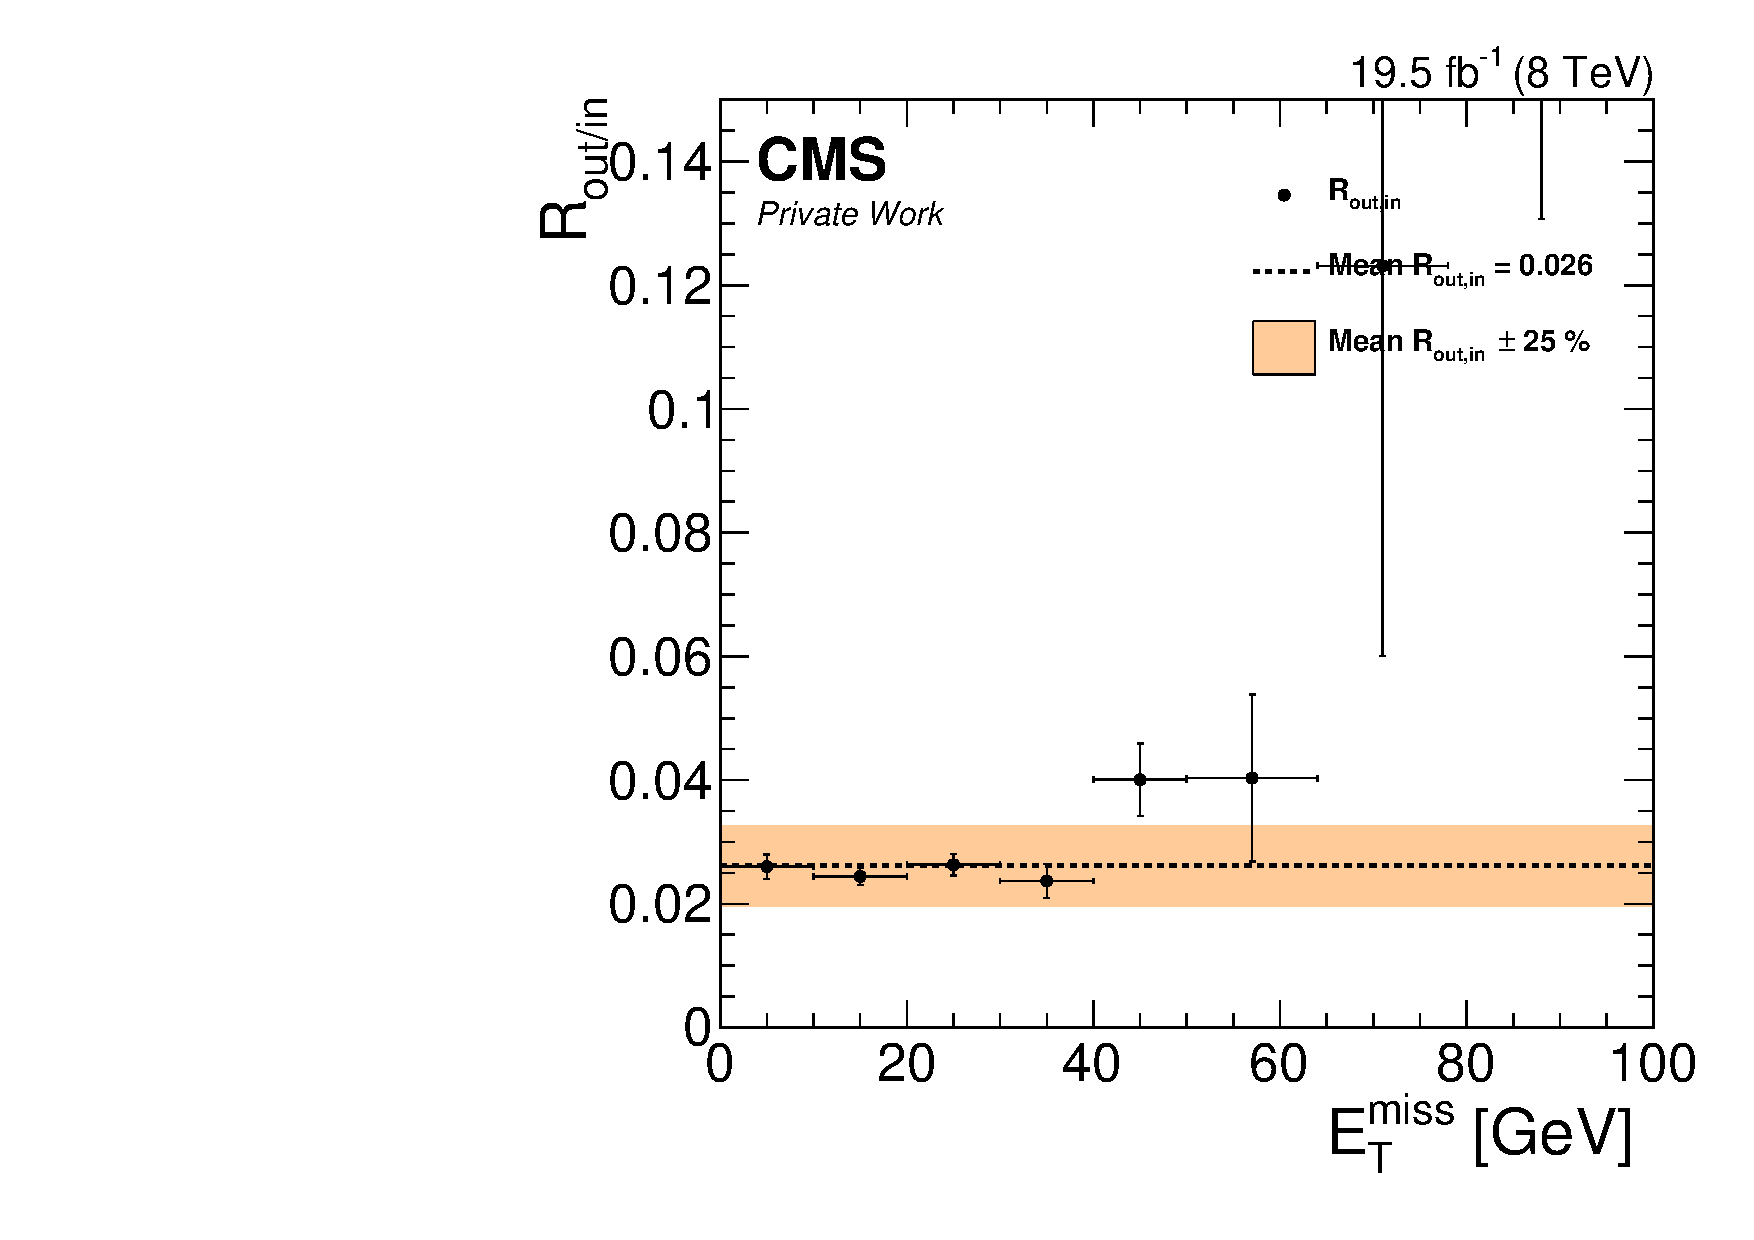
\includegraphics[width=\textwidth]{plots/BG/rOutIn/rOutInSyst_DrellYanControlForward_Full2012_MET_HighMass_MM_None.pdf}
\end{minipage}
\begin{minipage}[t]{0.49\textwidth}
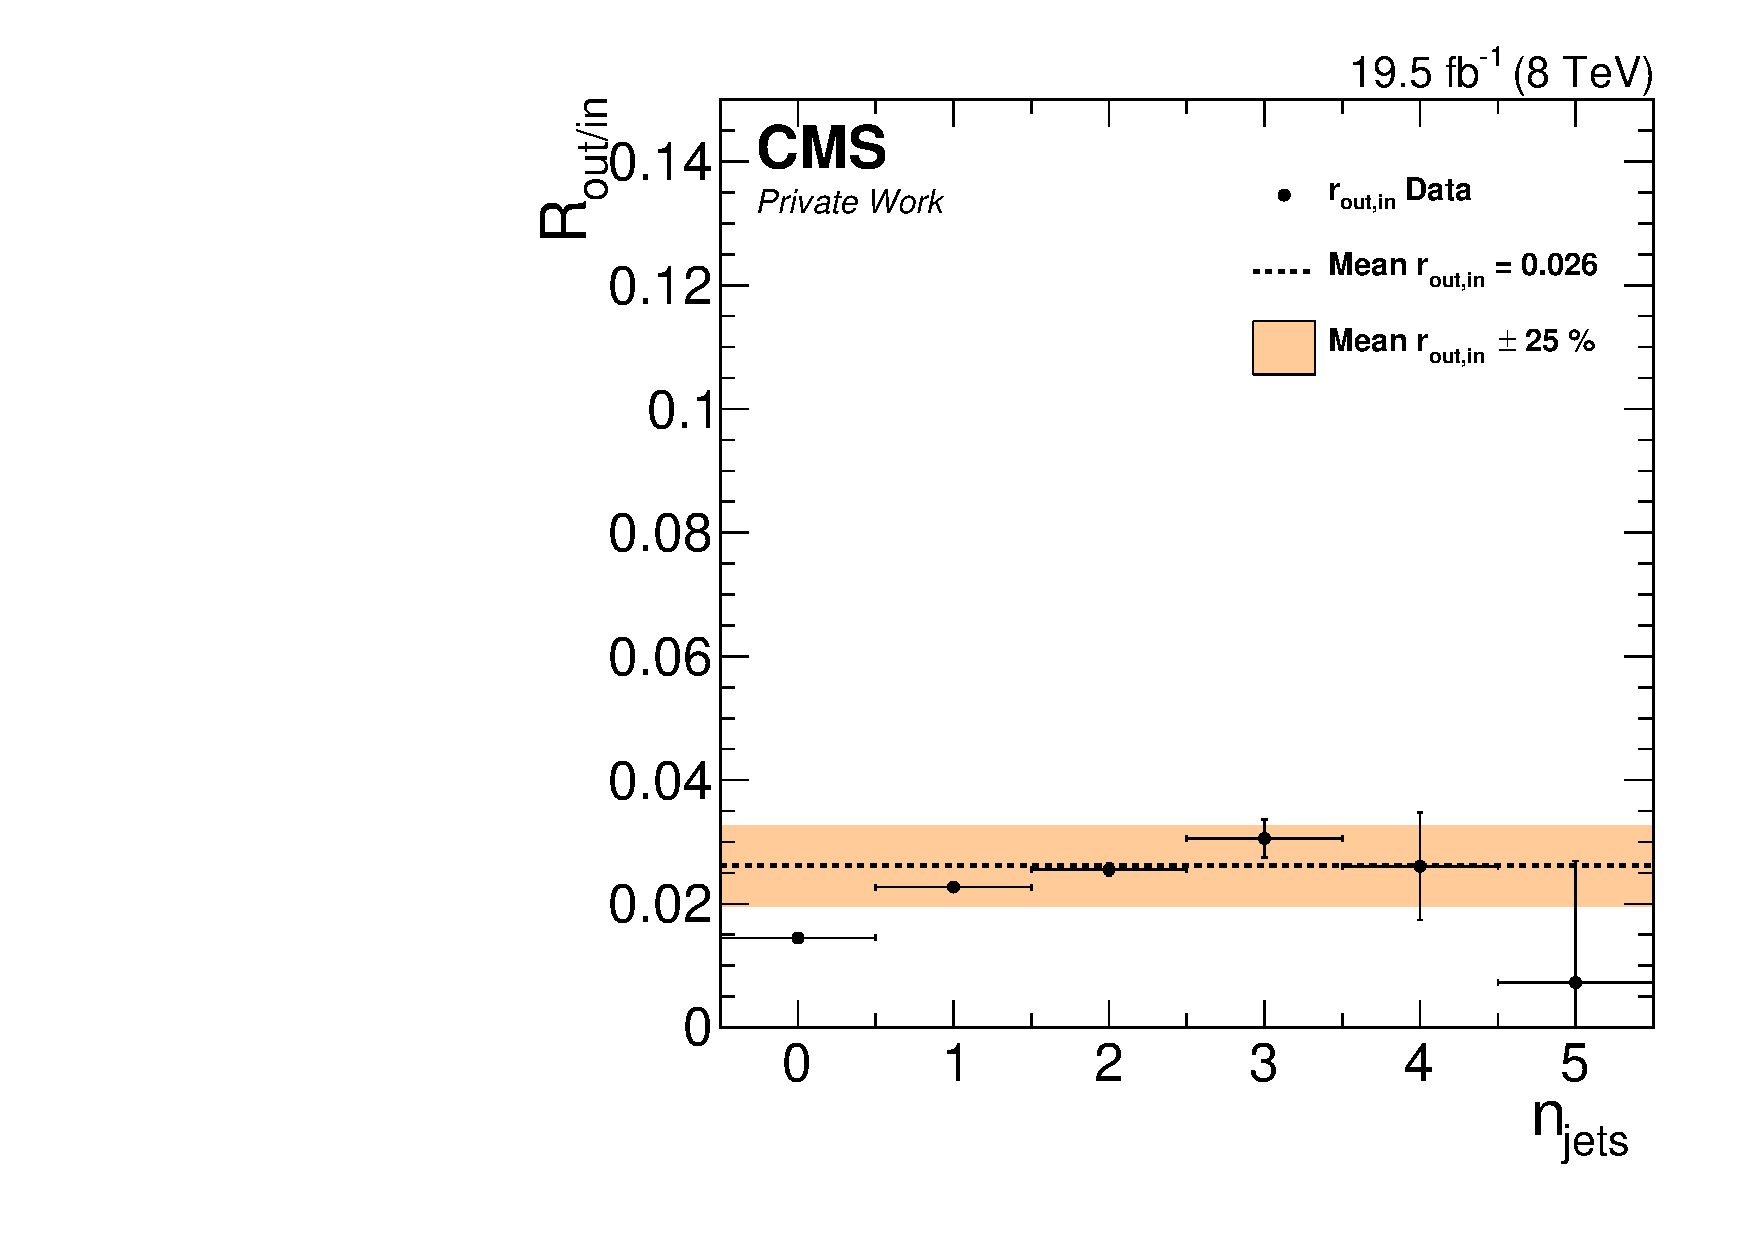
\includegraphics[width=\textwidth]{plots/BG/rOutIn/rOutInSyst_DrellYanControlForward_Full2012_NJets_HighMass_MM_None.pdf}
\end{minipage}
\caption{Dependencies of \Routin for the high-mass region on \MET (left) and \njets (right) for the central (top) and forward (bottom) lepton selection for \MM lepton pairs. The results on data are shown in black. The central value is shown as a black dashed line while the systematic uncertainty is shown as an orange band.}
\label{fig:ROutInDependencies6}
\end{figure} 